% Madrid Rental Market Analysis Report
% MBDS Machine Learning I — Group 8
% Overleaf-ready two-column IEEE-style layout
\documentclass[10pt,a4paper,twocolumn]{article}

% ─── Packages ────────────────────────────────────────────────────────────────
\usepackage[utf8]{inputenc}
\usepackage[T1]{fontenc}
\usepackage{helvet}                       % Arial-like sans serif
\renewcommand{\familydefault}{\sfdefault}
\usepackage[top=1.8cm,bottom=2cm,left=1.6cm,right=1.6cm]{geometry}
\usepackage{graphicx}
\usepackage{booktabs}
\usepackage{tabularx}
\usepackage{multirow}
\usepackage{xcolor}
\usepackage{hyperref}
\usepackage{caption}
\usepackage{subcaption}
\usepackage{float}
\usepackage{enumitem}
\usepackage{amsmath}
\usepackage{fancyhdr}
\usepackage{titlesec}
\usepackage{setspace}
\usepackage{colortbl}
\usepackage{array}

% ─── Colors ──────────────────────────────────────────────────────────────────
\definecolor{mbdsblue}{HTML}{1A3C6E}
\definecolor{accentblue}{HTML}{636EFA}
\definecolor{accentred}{HTML}{EF553B}
\definecolor{accentgreen}{HTML}{00CC96}
\definecolor{accentpurple}{HTML}{AB63FA}
\definecolor{lightgray}{HTML}{F5F5F5}
\definecolor{tabheader}{HTML}{D5E8F0}
\definecolor{passgreen}{HTML}{27AE60}
\definecolor{rowgreen}{HTML}{D5F0D5}
\definecolor{rowpink}{HTML}{FFD5D5}

% ─── Formatting ──────────────────────────────────────────────────────────────
\hypersetup{colorlinks=true,linkcolor=mbdsblue,urlcolor=accentblue,citecolor=mbdsblue}
\setlength{\columnsep}{0.6cm}
\setlength{\parindent}{0pt}
\setlength{\parskip}{4pt}
\setlist[itemize]{nosep,leftmargin=1.2em,topsep=2pt}
\setlist[enumerate]{nosep,leftmargin=1.5em,topsep=2pt}
\captionsetup{font=small,labelfont=bf,skip=4pt}

% Section formatting — compact
\titleformat{\section}{\large\bfseries\color{mbdsblue}}{\thesection.}{0.4em}{}[\vspace{-2pt}]
\titleformat{\subsection}{\normalsize\bfseries\color{mbdsblue}}{\thesubsection}{0.4em}{}[\vspace{-2pt}]
\titleformat{\subsubsection}{\small\bfseries\itshape}{\thesubsubsection}{0.4em}{}
\titlespacing*{\section}{0pt}{8pt}{4pt}
\titlespacing*{\subsection}{0pt}{6pt}{2pt}
\titlespacing*{\subsubsection}{0pt}{4pt}{2pt}

% Header/Footer
\pagestyle{fancy}
\fancyhf{}
\renewcommand{\headrulewidth}{0.4pt}
\fancyhead[L]{\small\color{mbdsblue}\textbf{Madrid Rental Market Analysis}}
\fancyhead[R]{\small\color{mbdsblue}MBDS --- Machine Learning I}
\fancyfoot[C]{\small\thepage}

% ─── Custom commands ─────────────────────────────────────────────────────────
\newcommand{\cluster}[1]{\textbf{C#1}}
\newcommand{\eur}[1]{€\,#1}
\newcommand{\sqm}{m\textsuperscript{2}}
\newcommand{\seg}[1]{\textit{#1}}          % cluster segment names in italic

% ═════════════════════════════════════════════════════════════════════════════
\begin{document}
\thispagestyle{empty}

% ─── TITLE BLOCK ─────────────────────────────────────────────────────────────
\twocolumn[{%
\begin{center}
\vspace{-0.5cm}
{\LARGE\bfseries\color{mbdsblue} \textbf{Location Over Space: Madrid's Rental Market Analysis}}\\[6pt]
{\large Clustering Segmentation and Regression Pricing Model}\\[8pt]
\rule{0.6\textwidth}{0.5pt}\\[6pt]
{\small
\textbf{Group 8:} Alberto Cabezudo Rodr\'iguez, Madelyn Ehni, Gilles Hamers,\\
Nicol\'as A.\ Higuera Wilches, Salah Mneimne\\[4pt]
Machine Learning I \hspace{1cm} February 28, 2026}
\end{center}
\vspace{0.3cm}
}]

% ─── EXECUTIVE SUMMARY ──────────────────────────────────────────────────────
\section*{Executive Summary}

This report presents a two-phase machine learning analysis of rental listings from \textit{Idealista.com} across Madrid. In \textbf{Phase 1}, a K-Means\footnote{\textbf{K-Means:} Unsupervised algorithm that partitions observations into $K$ groups by minimizing squared distances to cluster centroids.} clustering model segments properties into structurally distinct sub-markets based on the number of bedrooms and floor level, achieving four well-defined property 'profiles' (Silhouette\footnote{\textbf{Silhouette score:} Ranges from $-1$ to $+1$; measures how similar each observation is to its own cluster vs.\ the nearest alternative. Values above 0.4 indicate meaningful structure.} = 0.455). In \textbf{Phase~2}, a linear regression model estimates rental prices within the largest segment, \seg{Compact Traditional}, which represents $\approx$43\% of listings. This model achieved an $R^2$\footnote{\textbf{R\textsuperscript{2} (Coefficient of Determination):} Proportion of rent variation explained by the model; 0.644 means 64.4\% of price differences are accounted for by the predictors.} of 0.644 and MAPE\footnote{\textbf{MAPE (Mean Absolute Percentage Error):} Average prediction error as a percentage of actual value. A MAPE of 20\% means predictions are, on average, within 20\% of the true rent.} below 20\% across training, testing, and reserved datasets. Together, they answer two key questions for every listing: which market segment it belongs to, and what it should rent for.

Madrid’s rental market is made up of four distinct sub-markets. The clustering analysis revealed that property type and floor level define the market structure more clearly than any combination of amenities. Our resulting segments span a \eur{1,300} median monthly rent range with \seg{Compact Traditional} properties anchoring the majority of the market, followed by \seg{Small High-Rise Modern} properties with a 27\% median rent premium over it, even with an identical number of bedrooms. This gap is driven by floor-level and building modernity. At the top of the market, \seg{Large Low-Rise Family} and \seg{Large High-Rise Executive} residences share a median rent price of \eur{2,300} and \eur{2,400} but serve opposite tenant needs: garden access and suburban versus height, penthouse access and luxury districts. Pricing these two segments against a shared benchmark systematically misprices both.

Within the \seg{Compact Traditional} segment, the highest volume market, location is the dominant influence over rent, not size. The regression model shows that the marginal value of a square meter varies distinctly by district: in Salamanca, each additional m² is worth \eur{18.2} in rent, 2.5 times the \eur{7.4} baseline rate observed in peripheral districts. Outer districts such as Puente de Vallecas carry a structural discount regardless of property attributes. An identical 70~m$^{2}$ property can cost \eur{300}--\eur{400} more per month just based on neighborhood. Model performance is stable across training, testing, and hold-out sets, confirming that its pricing predictions will hold on new listings, not just the data it was trained on.


% ─── 1. DATA & METHODOLOGY ──────────────────────────────────────────────────
\section{Data \& Methodological Framework}

\subsection{Data Audit \& Cleaning}

The raw dataset contains 15 variables and 2,089 observations. Five variables carried missing values, three reported extreme values (outliers), and one registered a potential data-entry error.

Listings with missing values for Bedrooms and Floor were imputed using a 'contextual' median, based on their respective District and Area to preserve neighborhood-specific building patterns. Meanwhile, missing values for Elevator and Outer were handled using mode imputation.

Extreme values or outliers were defined using the IQR\footnote{\textbf{IQR (Interquartile Range):} Difference between the 75th and 25th percentiles. Values beyond $1.5\times$ IQR above Q3 are flagged as outliers.} method. Listings with extreme rent prices and floor areas were capped with upper limits of \eur{4,825} and 270~m$^{2}$ respectively, and bedrooms count was capped at four. Finally, a floor value of 43,039 (an obvious data-entry error) was flagged and treated as a missing value.

A full summary of quality issues and corrective actions is provided in Table~\ref{tab:cleaning}.
\subsection{Clustering Variable Selection}

Seven candidate variables were identified (see Annex~1). Here is what we discovered:

\textbf{Rent and District were excluded from the clustering:} Rent serves as the objective for the Phase 2 regression analysis. Including either option would distort segmentation in favor of pricing results, as the district anticipates regression. 

\textbf{Multicollinearity screening revealed a strong correlation between Bedrooms and square meters} (r=0.755; VIF\footnote{\textbf{VIF (Variance Inflation Factor):} Quantifies how much a predictor's variance is inflated by collinearity with other predictors. VIF $<5$ is acceptable; VIF $\geq10$ requires removal.} $\approx$ 9) as shown in Table~\ref{tab:vif}. Bedrooms + Floor (VIF 2.29) and Sq.Mt. + Floor (VIF 2.09) emerged as the two most effective combinations. Given that bedrooms serve as the main filter for tenant searches and exhibited the highest silhouette score (0.4552 compared to 0.4053), we opted for Bedrooms + Floor.

Finally, binary amenities (Elevator, Outer, Penthouse, Cottage) showed 3--5$\times$ standard-deviation separation after standardization. Including them produced \textit{dominated clusters}. Including individual amenities rather than focusing on market structure will lead to the formation of risk clusters, so they were kept as profiling variables.

% ─── 2. TECHNICAL APPROACH ──────────────────────────────────────────────────
\section{Technical Approach}

\subsection{Algorithm Choice \& K Selection}

K-Means was chosen for three reasons: \textbf{(a)} The clusters are interpretable. A 3.5-bedroom centroid on floor 6.7 communicates a real property type. \textbf{(b)} The model is fully reproducible on updated listings at any time and get consistent, comparable segments. \textbf{(c)} Each property's cluster label is used to filter the dataset, so the regression model trains only on properties from that segment.

All variables were standardized (z-score) before fitting. The number of potential groups or clusters ($K$) was evaluated from 2 to 7 using four metrics: Inertia, Silhouette, Calinski-Harabasz, Davies-Bouldin. Full results are shown in Table~\ref{tab:kmetrics}.

$K\!=\!3$ delivers the highest Silhouette (0.460) but merges the Large High-Rise Executive and Large Low-Rise Family segments. However, $K\!=\!4$ (Silhouette 0.455) was selected because it preserves the structural distinction between large high-rise and large low-rise properties. The 0.0047 Silhouette trade-off is commercially justified. 

\subsection{Scenario Testing}

As illustrated in Table~\ref{tab:scenarios}, we tested twelve different variable combinations at K=4 to verify whether binary amenities should be included in the clustering. The silhouette score, variance inflation factor (VIF), cluster balance (minimum/maximum percentage), and a domination check were used to evaluate each scenario.

While several scenarios (3--12) show relatively high silhouette values, this enhancement is misleading. In such cases, the algorithm categorizes listings mainly by whether that specific feature is present or absent, rather than following a logical market structure, as the distance calculation is largely influenced by a binary amenity. 

This is particularly clear in Scenario 7, where 68.4\% of the observations converge into one cluster. Only Scenario 1 yields segments that are both economically interpretable and balanced, all while fulfilling the necessary validation criteria.

% ─── 3. SEGMENTATION RESULTS ────────────────────────────────────────────────
\section{Segmentation Results}

\subsection{Model Validation}

The final model was validated across four independent validation criteria (n (\%), Silhouette, Negative Silhouette, Rent CV ($\sigma/\mu$)) before any business interpretation was applied and can be found in Table~\ref{tab:validation_annex}.
\begin{table}[H]
\centering
\caption{Cluster validation summary ($K\!=\!4$, Silhouette = 0.455).}
\label{tab:validation}
\small
\setlength{\tabcolsep}{3pt}
\begin{tabular}{@{}lcccl@{}}
\toprule
\textbf{Cluster} & \textbf{n (\%)} & \textbf{Sil.} & \textbf{Rent CV} & \textbf{Bal.} \\
\midrule
\cluster{0} Large Hi-Rise Exec. & 229 (11.0\%) & 0.370 & 0.478 & \textcolor{passgreen}{PASS} \\
\cluster{1} Compact Traditional & 903 (43.2\%) & 0.476 & 0.532 & \textcolor{passgreen}{PASS} \\
\cluster{2} Large Lo-Rise Family & 624 (29.9\%) & 0.489 & 0.537 & \textcolor{passgreen}{PASS} \\
\cluster{3} Small Hi-Rise Modern & 333 (15.9\%) & 0.394 & 0.487 & \textcolor{passgreen}{PASS} \\
\bottomrule
\end{tabular}
\end{table}

All four clusters meet the validation checks. Rent dispersion remains stable (CV between 0.478 and 0.537), only one listing shows a negative silhouette, and cluster sizes are well balanced. In simpler terms, almost every property sits closest to its assigned centroid. 

\cluster{1} (\seg{Compact Traditional}) represents 43.2\% of all listings, has zero negative silhouettes, and a silhouette score of 0.476. Its rent dispersion ($\sigma$ €677; CV 0.532) is substantial, making it the most commercially relevant segment for Phase 2 regression modeling. 

What is also noticeable is that the median rents confirm a clear price tier separation within a range of \eur{1,300}: The lowest is \cluster{1} at \eur{1,100}, followed by \cluster{3} at \eur{1,400} (+27\%), then \cluster{2} at \eur{2,300} (+64\%) and \cluster{0} with a median rent of \eur{2,400}.


\subsection{Cluster Profiles}

The 2$\times$2 matrix below captures the structural segmentation logic of the 4 clusters within two dimensions: Unit size (compact $\leq$2 beds vs. large $\geq$3 beds) and floor level (low-rise $\leq$4 vs. high-rise $\geq$5). Detailed Cluster Profiles, Pricing Mechanisms and Tenant Personas are reported in Table~\ref{tab:profiles} to support the interpretation.

\begin{table}[H]
\centering
\caption{Segmentation matrix: 4 clusters in 2 dimensions.}
\label{tab:matrix}
\small
\setlength{\tabcolsep}{3pt}
\begin{tabular}{@{}p{1.4cm}|p{3.0cm}|p{3.0cm}@{}}
\toprule
 & \textbf{Low-Rise ($\bar{F}\!\approx\!2$)} & \textbf{High-Rise ($\bar{F}\!\approx\!6.7$)} \\
\midrule
\textbf{Large} \newline (3--4 beds) &
  \cluster{2} \textit{Lg.\ Low-Rise Family} \newline
  $n\!=\!624$ (29.9\%) \newline
  Med.\ rent \eur{2,300} \newline
  \eur{13.7}/\sqm{} \textbar{} Cottage 13\% &
  \cluster{0} \textit{Lg.\ Hi-Rise Exec.} \newline
  $n\!=\!229$ (11.0\%) \newline
  Med.\ rent \eur{2,400} \newline
  \eur{15.0}/\sqm{} \textbar{} Penthouse 20\% \\
\midrule
\textbf{Compact} \newline (1--2 beds) &
  \cluster{1} \textit{Compact Traditional} \newline
  $n\!=\!903$ (43.2\%) \newline
  Med.\ rent \eur{1,100} \newline
  \eur{16.2}/\sqm{} \textbar{} Elev.\ 82\% &
  \cluster{3} \textit{Small Hi-Rise Modern} \newline
  $n\!=\!333$ (15.9\%) \newline
  Med.\ rent \eur{1,400} \newline
  \eur{17.7}/\sqm{} \textbar{} Penthouse 23\% \\
\bottomrule
\end{tabular}
\end{table}
\textbf{Selected segment profile:} \seg{Compact Traditional} (\cluster{1}) listings cover smaller apartments on lower floors in older city buildings, many without full lift access. This is the most common segment in the market. Rents are relatively affordable in total, but expensive per square meter because of the central location. What matters most here is the street and neighborhood, not extra space or luxury features. This cluster was selected for our regression model for three reasons: It represents 43.2\% of all listings, it carries the highest within-segment rent dispersion (CV = 0.532, $\sigma$ = €677), and its €16.2/m$^{2}$ price intensity points to a location-driven pricing pattern that a district-aware model can directly exploit.

\subsection{Business Interpretation}

\textbf{(a)~\seg{Compact Traditional} \cluster{1} is the agency's most important segment.} At 43.2\% of all listings, it's the most common category on any platform. An apartment in Centro costs between €300 and €400 more per month than an identical apartment in Vallecas, despite a median rent of €1,100 and a standard deviation of €677. However, without a model that accounts for district variations, apartment prices are similar. Compact Traditional apartments' price intensity of €16.2/m$^{2}$ outperforms the two larger unit segments, C2 at €13.7/m$^{2}$ and C0 at €15.0/m$^{2}$, as tenants prioritize central location over space. 

\textbf{(b)~\seg{Large High-Rise Executive} (\cluster{0}) and \seg{Low-Rise Family} (\cluster{2}) share a price point but are opposite products.} In both clusters, 160~m$^{2}$ three-bedroom homes rent for €2,300--€2,400 per month. \cluster{0} offers remarkable height, stunning views, and a luxurious interior (Penthouse 19.7\%, Elevator 99.6\%, Floor mean 6.7, Salamanca/Chamartín). \cluster{2} has garden access and suburban dimensions (Moncloa/Hortaleza, Cottage 13.1\%, Floor mean 2.3). Using a large-unit benchmark for both will misprice one. All of this shows that $K\!=\!4$ emphasizes this difference, while $K\!=\!3$ minimizes it. 

\textbf{(c)~\seg{Small High-Rise Modern} (\cluster{3}) vs.\ \seg{Compact Traditional} (\cluster{1}) reveals the floor premium.} Both clusters have a median of 2 bedrooms, yet \cluster{3} rents for €1,400/month vs. \cluster{1}'s €1,100/month, which is a 27.3\% premium attributable entirely to floor level (6.7 vs 2.1) and modernity. \cluster{3}'s €17.7/m$^{2}$ is the highest price intensity in the dataset. An agent benchmarking a \cluster{3} listing against a comparable \cluster{1} leaves roughly €300/month on the table per listing. The correct comparison is floor-matched, not bedroom-matched.

% ─── 4. LINEAR REGRESSION ───────────────────────────────────────────────────
\section{Linear Regression Model}

\subsection{Scope \& Setup}

For the linear regression model, we focus on \cluster{1} (\seg{Compact Traditional}), which includes 903 properties ($\approx$43\% of the dataset), making it the largest and most statistically robust segment. This cluster is characterized by compact apartments, typically with one or two bedrooms and located on relatively low-to-mid floors. Compared to other clusters, it combines a high number of observations with moderate dispersion in rental prices, providing a stable basis for modeling and reducing structural heterogeneity (see Table~\ref{tab:validation}).

Non-predictive columns are then removed, including Id, Address, Number, Area, and property-type variables such as Cottage and Semidetached, which either lack explanatory value or are not representative within this cluster. The remaining variables are classified as continuous (e.g., Sq.Mt, Bedrooms, Floor) or binary (e.g., Outer, Elevator, Penthouse, Duplex). Histograms show moderately right-skewed distributions in size and rent, typical of housing markets, but without extreme tails after outlier treatment (see Figure~\ref{fig:hist_cont}). Binary variables display sufficient variability to contribute meaningfully to regression estimation (see Figure~\ref{fig:hist_bin}).

Finally, special treatment is applied to District. To avoid unstable coefficients from sparsely represented locations, districts with fewer than 25 listings are grouped into an “Other” category (see Table~\ref{tab:districts}). One-hot encoding with a reference district is then implemented, ensuring interpretability while preventing multicollinearity. At this point, the dataset is structurally consistent and ready for OLS\footnote{\textbf{OLS (Ordinary Least Squares):} Linear regression method that estimates coefficients by minimizing the sum of squared residuals between observed and predicted values.} modeling.


\subsection{Model Building \& Selection}

To ensure robust evaluation, the dataset is divided into three subsets: 10\% is set aside as a reserved (hold-out) set, while the remaining 90\% is split equally into training and testing sets. The training set is used for estimation and specification adjustments; the testing set evaluates intermediate refinements, and the reserved set provides a final unbiased assessment. This structure allows us to prevent overfitting and improves generalization reliability. 

The baseline OLS model with all predictors achieved $R^2\!=\!0.627$ (Adj.\ $R^2\!\approx\!0.607$), explaining a substantial share of rent variation within \cluster{1} (see Table~\ref{tab:ols_initial}). Bedrooms and Floor, our clustering variables, were dropped with virtually no $R^2$ loss ($\approx$0.626), confirming their limited variability within the cluster (see Table~\ref{tab:ols_dropped}).

Multicollinearity is assessed through the pairwise correlation matrix and Variance Inflation Factor (VIF), with a VIF threshold of 10, indicating acceptable levels as shown in Table~\ref{tab:vif_reg}.

Feature selection via RFECV\footnote{\textbf{RFECV (Recursive Feature Elimination with Cross-Validation):} Iteratively removes the least important predictor and uses cross-validation to identify the optimal feature subset.} reduced the model to 17 predictors; backward elimination further removed non-significant district dummies such as Hortaleza and Ciudad Lineal.

To enhance interpretability, interaction terms between Sq.Mt and District are introduced. These allow the marginal effect of size to vary by location, capturing spatial heterogeneity. The final model improves to an $R^2$ of 64.4\%, with adjusted $R^2$ closely aligned, indicating genuine explanatory gains rather than overfitting. Districts such as Puente de Vallecas and the grouped Other category show negative base effects, while several central districts display positive size interaction effects, meaning square meters are valued differently across locations (Table~\ref{tab:ols_final}).
 
\subsection{Final Model and Performance Metrics}

The final model retains 10 features: Sq.Mt, Outer, two district dummies (Other, Puente Vallecas), and six Sq.Mt~$\times$~District interactions. The implications of the model's output are discussed in the next section.

\begin{table}[H]
\centering
\caption{Final OLS model — coefficient estimates (Cluster~1, $n_{\text{train}}\!=\!406$).}
\label{tab:ols_coeffs}
\small
\setlength{\tabcolsep}{4pt}
\begin{tabular}{@{}l r r r c@{}}
\toprule
\textbf{Predictor} & \textbf{$\hat{\beta}$} & \textbf{Std.\ Err.} & \textbf{$t$} & \textbf{Sig.} \\
\midrule
\rowcolor{lightgray}
\multicolumn{5}{@{}l}{\textit{Base predictors}} \\
Intercept              & 375.39 & 63.26 &  5.94 & *** \\
Sq.Mt (m\textsuperscript{2}) &   7.38 &  0.95 &  7.78 & *** \\
Outer (exterior unit)  & 107.27 & 51.84 &  2.07 & *   \\
District: Other        &$-$214.98 & 79.51 & $-$2.70 & **  \\
District: Puente Vallecas &$-$199.91 & 99.25 & $-$2.01 & *   \\
\midrule
\rowcolor{lightgray}
\multicolumn{5}{@{}l}{\textit{Sq.Mt $\times$ District interactions (marginal €/m\textsuperscript{2} over baseline)}} \\
$\times$ Centro        &  6.03 & 0.73 &  8.31 & *** \\
$\times$ Chamart\'in   &  3.79 & 0.99 &  3.85 & *** \\
$\times$ Chamber\'i    &  5.78 & 0.96 &  6.02 & *** \\
$\times$ Moncloa       &  3.22 & 1.41 &  2.28 & *   \\
$\times$ Retiro        &  4.26 & 1.20 &  3.57 & *** \\
$\times$ Salamanca     & 10.85 & 0.83 & 13.12 & *** \\
\midrule
\multicolumn{5}{@{}l}{\scriptsize *** $p<0.001$\quad ** $p<0.01$\quad * $p<0.05$} \\
\multicolumn{5}{@{}l}{\scriptsize $R^2\!=\!0.644$, Adj.\ $R^2\!=\!0.635$, $F(10,\,395)\!=\!71.53$, $p<0.001$} \\
\bottomrule
\end{tabular}
\end{table}
\begin{table}[H]
\centering
\caption{Regression performance across data splits.}
\label{tab:regression}
\small
\begin{tabular}{@{}lcccc@{}}
\toprule
\textbf{Metric} & \textbf{Train} & \textbf{Test} & \textbf{Reserved} \\
\midrule
$R^2$ & 0.644 & 0.644 & 0.630 \\
MAE (\eur{}) & 260 & 267 & 242 \\
RMSE (\eur{}) & 391 & 426 & 364 \\
MAPE (\%) & 19.7 & 20.2 & 19.2 \\
\bottomrule
\end{tabular}
\end{table}

\subsection{Model Interpretation}
\textbf{The model explains nearly two-thirds of rent variation within \seg{Compact Traditional}.} An R\textsuperscript{2} of 0.644 means that district, size, and their interaction together account for 64.4\% of the price differences observed across these properties. The remaining 35.6\% reflects factors the model cannot observe from a listing alone such as interior quality, renovation standard, specific floor orientation, and landlord negotiation.

The model's coefficients reveal the pricing mechanics of Madrid's \seg{Compact Traditional} market:

\begin{itemize}
\item \textbf{Base rate:} \eur{375}/mo for a hypothetical 0~\sqm{} non-exterior unit in the reference district---the intercept anchors the model.
\item \textbf{Size premium:} Each additional \sqm{} raises average rent prices by \eur{7.4} in the reference district, holding other attributes constant.  
\item \textbf{Location multiplier (Sq.Mt $\times$ District):} Not only size matters, location is key. The increase in monthly rent for an additional \sqm changes significantly across districts. The total value of this increase equals the baseline (\eur{7.38}) plus the district's interaction. Salamanca leads with a marginal value of (\eur{10.8}/\sqm{}) on top of the base, followed by Centro (+\eur{6.0}) and Chamber\'i (+\eur{5.8}). A 70~\sqm{} flat in Salamanca is predicted at $\sim$\eur{1,650}, vs.\ $\sim$\eur{890} in the reference district, an 85\% location premium.
\item \textbf{Peripheral discount:} In contrast, Puente Vallecas ($-$\eur{200}) and ``Other'' grouped districts ($-$\eur{215}) carry negative base effects, reflecting lower demand.
\item \textbf{Exterior premium:} Outer-facing units add \eur{107} ($p\!=\!0.039$), a modest but significant amenity premium.
\end{itemize}

\textbf{The key insight:} Within \seg{Compact Traditional}, \textbf{location dominates size}. The same 70~\sqm{} unit can range from \eur{890} to \eur{1,650} depending on district, a spread larger than what any physical feature can produce. This confirms the clustering finding that \cluster{1} \textbf{tenants ``pay for address, not space''.}

The model will perform as reliably on new listings as it does on the data it was trained on (see Figure~\ref{fig:rvf_train}). R\textsuperscript{2} holds at 0.64 across training and test sets and falls only to 0.63 on the reserved hold-out. Predictions will not deteriorate as new listings enter the portfolio.

% ─── 5. CONCLUSION ──────────────────────────────────────────────────────────
\section{Conclusion \& Recommendations}

\textbf{The Madrid rental market is segmented, not continuous.} Treating all listings as a single market creates systematic pricing errors. The segmentation identifies four discrete property types with distinct price dynamics. The \seg{Compact Traditional} segment accounts for 43\% of all listings and should anchor the agency's volume strategy. It is large enough to justify a dedicated pricing process and small enough to model with precision.

\textbf{Where a property is located matters more than how big it is.} Within the \seg{Compact Traditional} segment, district drives rent more than floor area. A square meter in Salamanca is \eur{10.85} above the base rate, nearly 2.5$\times$ the premium of a square meter in the average district. Pricing primarily by size leaves a margin on the table in premium locations and over-pricing in peripheral ones.

\textbf{Segment-first pricing prevents the errors a blended model cannot see.} Two segments (\cluster{0} and \cluster{2}) occupy the same price range with opposite profiles. A single-market model would average them out and produce wrong estimates for both. Segmenting first ensures the right pricing logic is applied to the right property type.

\subsection{Recommendations}
\begin{itemize}
    \item \textbf{Classify before you price.} Use the clustering model to assign each new listing to a segment, then apply the corresponding regression model. A one-step pricing tool built on a blended model will underperform for most property types.
    \item \textbf{Use the model as a mispricing detector, not just a price setter.} Flag any listed property whose asking rent falls more than 1$\sigma$ below the model's prediction; these are the clearest candidates for upward renegotiation.
    \item \textbf{Treat the model's output as a floor, not a ceiling, at the top end.} Above \eur{2,000}/month the model under-predicts, because prestige-street effects and interior specification are not captured. For premium listings, use the predicted rent as the minimum justifiable price.
    \item \textbf{Extend the pipeline to the remaining three segments.} Dedicated regression models for C0, C2, and C3 would cover the remaining 57\% of the portfolio with the same precision achieved here for C1.
\end{itemize}




% _____________________________________________________________________



% ANNEX (start new page, switch to single-column for full-width figures)

\onecolumn
\newpage
\thispagestyle{fancy}

\setlength{\textfloatsep}{4pt plus 2pt minus 2pt}
\setlength{\floatsep}{4pt plus 2pt minus 2pt}
\setlength{\intextsep}{4pt plus 2pt minus 2pt}
\titlespacing*{\subsection}{0pt}{6pt}{3pt}

% Reset counters for annex numbering (A1, A2, ...)
\setcounter{table}{0}
\renewcommand{\thetable}{A\arabic{table}}
\setcounter{figure}{0}
\renewcommand{\thefigure}{A\arabic{figure}}

\begin{center}
{\Large\bfseries\color{mbdsblue} Technical Annex}\\[2pt]
\rule{0.5\textwidth}{0.4pt}
\end{center}
\vspace{0.1cm}

\subsection*{Annex 0 --- Data Cleaning Summary}
\begin{table}[H]
\centering
\caption{Data quality issues and corrective actions.}
\label{tab:cleaning}
\small
\begin{tabularx}{\textwidth}{@{}lXlX@{}}
\toprule
\textbf{Variable} & \textbf{Issue} & \textbf{Scale} & \textbf{Resolution} \\
\midrule
Floor & Entry error: value = 43,039 & 1 record & Set to missing; contextual median imputation \\
Rent & Right-skewed; max \eur{16,000} & 114 rows (5.5\%) & IQR cap at \eur{4,825} \\
Sq.Mt & Right-skewed; max 1,250~\sqm{} & 188 rows (9.0\%) & IQR cap at 270~\sqm{} \\
Bedrooms & Outliers up to 8; 89 missing & 162 capped; 89 imputed & Cap at 4; contextual median (District+Area) \\
Floor & 142 missing post error fix & 142 rows (6.8\%) & Contextual median: Dist.+Area $\to$ Dist.\ $\to$ Global \\
Elevator / Outer & 133 / 162 missing & 6.4\% / 7.8\% & Mode imputation (both mode = 1) \\
\bottomrule
\end{tabularx}
\end{table}

% ─── ANNEX 1 ─────────────────────────────────────────────────────────────────
\subsection*{Annex 1 --- Data Audit \& Variable Selection}

\begin{figure}[H]
\centering
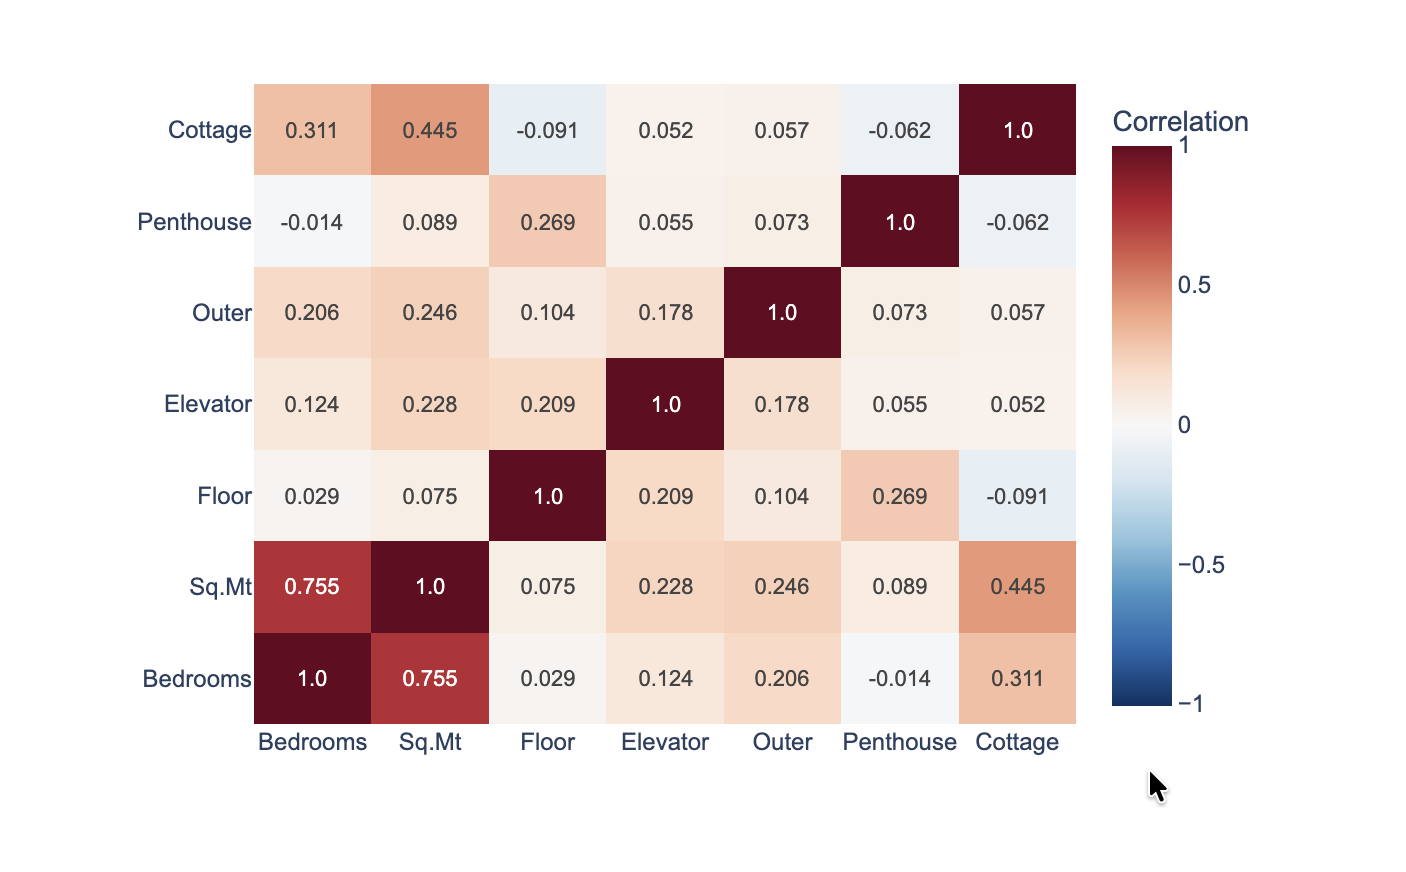
\includegraphics[width=0.85\linewidth]{figures/pairwise_correlation.png}
\caption{Pairwise correlation matrix for candidate
clustering variables. Strong correlation between Bedrooms and Sq.Mt
($r\!=\!0.755$) confirms their redundancy; Bedrooms and Floor
($r\!=\!0.044$) and Sq.Mt and Floor ($r\!=\!0.075$) are near-independent,
validating the final two-variable selection.}
\label{fig:corr}
\end{figure}

\begin{table}[H]
\centering
\caption{VIF screening of candidate variable combinations.}
\label{tab:vif}
\small
\begin{tabular}{@{}l l r c@{}}
\toprule
\textbf{Combination} & \textbf{Variable} & \textbf{VIF} & \textbf{Status} \\
\midrule

% ── Combination 1 ──
\rowcolor{lightgray}
\textbf{Bedrooms + Sq.Mt + Floor} & & \textit{max 9.88} & \\
\quad Bedrooms & & \textcolor{accentred}{9.88} & \textcolor{accentred}{$\uparrow$ high} \\
\quad Sq.Mt    & & \textcolor{accentred}{9.01} & \textcolor{accentred}{$\uparrow$ high} \\
\quad Floor    & & \textcolor{passgreen}{2.30} & \textcolor{passgreen}{ok} \\
\midrule

% ── Combination 2 ──
\rowcolor{lightgray}
\textbf{Bedrooms + Floor} & & \textit{max 2.29} & \\
\quad Bedrooms & & \textcolor{passgreen}{2.29} & \textcolor{passgreen}{ok} \\
\quad Floor    & & \textcolor{passgreen}{2.29} & \textcolor{passgreen}{ok} \\
\midrule

% ── Combination 3 ──
\rowcolor{lightgray}
\textbf{Sq.Mt + Floor} & & \textit{max 2.09} & \\
\quad Sq.Mt & & \textcolor{passgreen}{2.09} & \textcolor{passgreen}{ok} \\
\quad Floor & & \textcolor{passgreen}{2.09} & \textcolor{passgreen}{ok} \\

\bottomrule
\multicolumn{4}{@{}p{0.9\columnwidth}@{}}{\scriptsize
  \textit{Conclusion:} Bedrooms and Sq.Mt cannot coexist (VIF\,$>$\,5).
  Two viable base combinations advance to Stage~4: \textbf{Bedrooms + Floor} and
  \textbf{Sq.Mt + Floor}.
  Threshold: VIF\,$<$\,5 acceptable; VIF\,$<$\,10 tolerable.}\\
\end{tabular}
\end{table}


% ─── ANNEX 2 ─────────────────────────────────────────────────────────────────
\subsection*{Annex 2 --- Algorithm Choice, K Selection \& Scenario Testing}

\begin{table}[H]
\centering
\caption{Cluster validation metrics ($K\!=\!2$ to 7).}
\label{tab:kmetrics}
\small
\begin{tabular}{@{}cccccl@{}}
\toprule
\textbf{K} & \textbf{Inertia} & \textbf{Silhouette} & \textbf{Calinski-H.} & \textbf{Davies-B.} & \textbf{Decision} \\
\midrule
2 & 2,553 & 0.407 & 1,328 & 1.077 & Too coarse \\
3 & 1,461 & \textbf{0.460} & \textbf{1,939} & 0.790 & Statistically strongest \\
\rowcolor{tabheader} \textbf{4} & \textbf{1,127} & \textbf{0.455} & 1,880 & 0.837 & \textbf{SELECTED} \\
5 & 918 & 0.424 & 1,851 & 0.875 & Diminishing returns \\
6--7 & $<$769 & $<$0.443 & $<$1,848 & $>$0.848 & Over-fragmented \\
\bottomrule
\end{tabular}
\end{table}

\begin{figure}[H]
\centering
\begin{subfigure}[t]{0.48\textwidth}
\centering
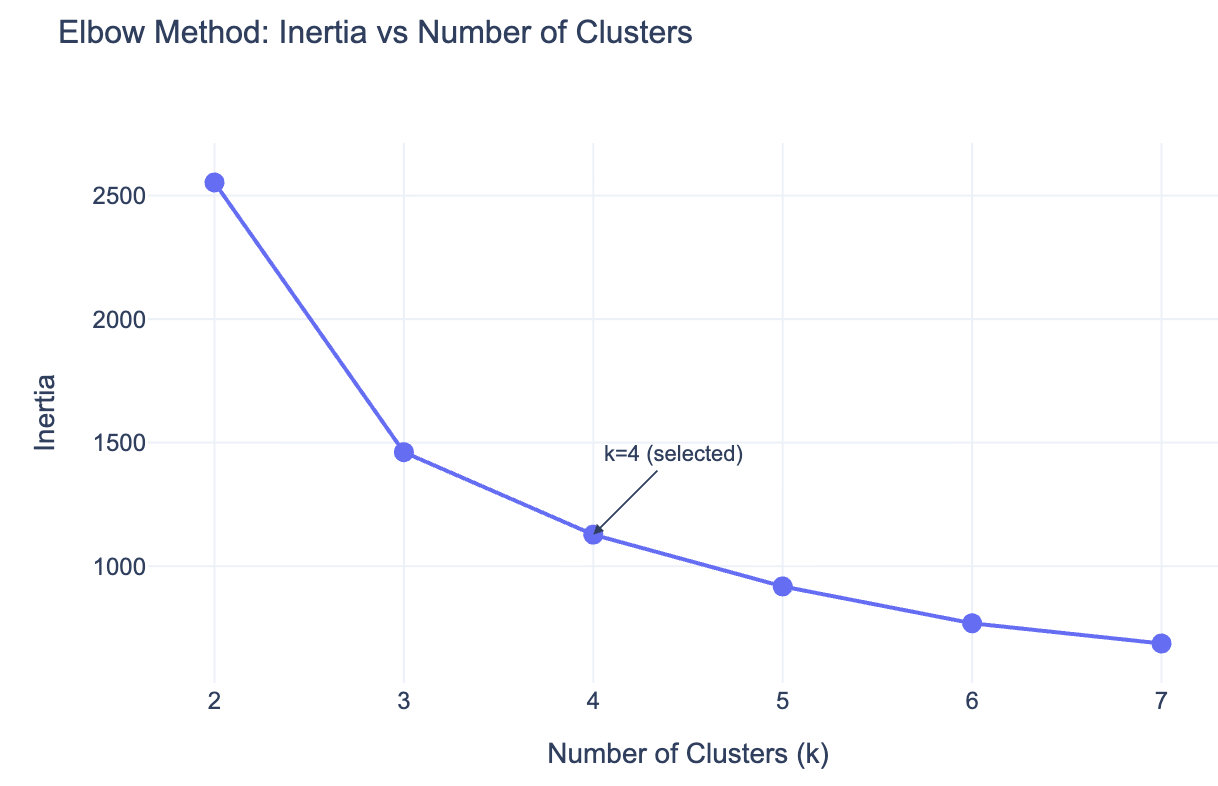
\includegraphics[width=\textwidth]{figures/elbow_method.png}
\caption{Elbow plot: Inertia vs.\ $K$.}
\end{subfigure}
\hfill
\begin{subfigure}[t]{0.48\textwidth}
\centering
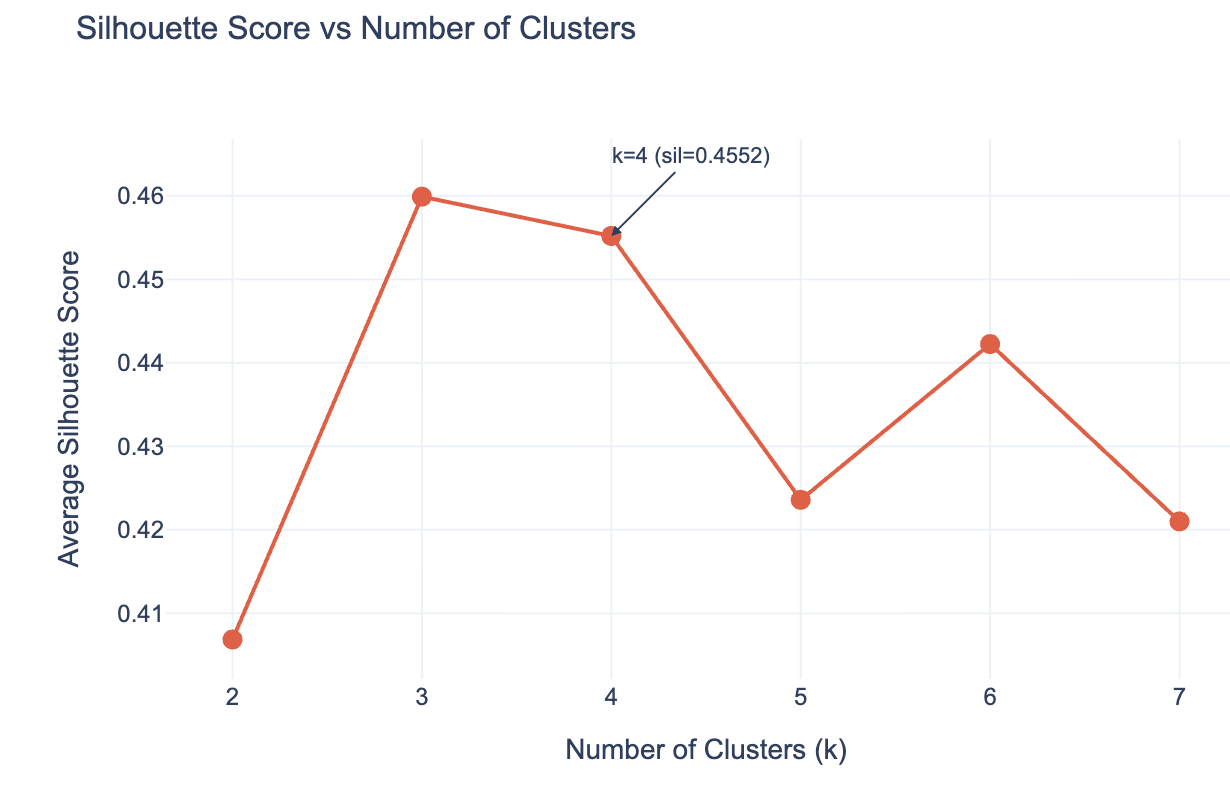
\includegraphics[width=\textwidth]{figures/silhouette.png}
\caption{Silhouette and additional metrics vs.\ $K$.}
\end{subfigure}
\caption{K-selection diagnostic plots.}
\label{fig:kselection}
\end{figure}

\begin{table}[H]
\centering
\caption{Twelve-scenario variable-combination testing at $K\!=\!4$.
\textit{Green} = selected \textbar{} \textit{Pink} = dominated cluster detected.}
\label{tab:scenarios}
\small
\setlength{\tabcolsep}{5pt}
\begin{tabularx}{\textwidth}{@{} c X c c c c c c @{}}
\toprule
\textbf{\#} & \textbf{Variable Combination} & \textbf{Vars} &
\textbf{Silhouette} & \textbf{VIF\textsubscript{max}} &
\textbf{Min Cluster} & \textbf{Max Cluster} & \textbf{Dominated} \\
\midrule
\rowcolor{lightgray}
\multicolumn{8}{@{}l}{\textit{\small Bedrooms-based combinations}} \\
\rowcolor{rowgreen}
1 & Bedrooms + Floor                 & 2 & \textbf{0.4552} & 2.29 & 11.0\% & 43.2\% & \textcolor{passgreen}{No}  \\
\rowcolor{rowpink}
2 & Bedrooms + Floor + Elevator      & 3 & 0.4751 & 5.63 & 11.2\% & 37.4\% & \textcolor{accentred}{Yes} \\
\rowcolor{rowpink}
3 & Bedrooms + Floor + Outer         & 3 & 0.4718 & 5.46 & 12.3\% & 36.7\% & \textcolor{accentred}{Yes} \\
\rowcolor{rowpink}
4 & Bedrooms + Floor + Penthouse     & 3 & 0.4825 & 2.52 &  8.1\% & 43.7\% & \textcolor{accentred}{Yes} \\
\rowcolor{rowpink}
5 & Bedrooms + Floor + Cottage       & 3 & 0.4680 & 2.60 &  4.2\% & 45.4\% & \textcolor{accentred}{Yes} \\
\rowcolor{rowpink}
6 & Bedrooms + Floor + ALL amenities & 6 & 0.4812 & 7.25 &  4.2\% & 68.4\% & \textcolor{accentred}{Yes} \\
\midrule
\rowcolor{lightgray}
\multicolumn{8}{@{}l}{\textit{\small Sq.Mt-based combinations}} \\
7  & Sq.Mt + Floor                    & 2 & 0.4053 & 2.09 & 13.6\% & 34.5\% & \textcolor{passgreen}{No}  \\
\rowcolor{rowpink}
8  & Sq.Mt + Floor + Elevator         & 3 & 0.5092 & 5.02 & 11.2\% & 47.4\% & \textcolor{accentred}{Yes} \\
\rowcolor{rowpink}
9  & Sq.Mt + Floor + Outer            & 3 & 0.5089 & 4.60 & 12.3\% & 48.2\% & \textcolor{accentred}{Yes} \\
\rowcolor{rowpink}
10 & Sq.Mt + Floor + Penthouse        & 3 & 0.5180 & 2.24 &  8.1\% & 55.7\% & \textcolor{accentred}{Yes} \\
\rowcolor{rowpink}
11 & Sq.Mt + Floor + Cottage          & 3 & 0.5043 & 2.65 &  4.2\% & 56.2\% & \textcolor{accentred}{Yes} \\
\rowcolor{rowpink}
12 & Sq.Mt + Floor + ALL amenities    & 6 & 0.5141 & 7.17 &  4.2\% & 77.1\% & \textcolor{accentred}{Yes} \\
\bottomrule
\multicolumn{8}{@{}p{\textwidth}@{}}{\scriptsize
\textit{Note:} Higher silhouette in scenarios 3--12 is misleading --- a binary amenity
dominates the distance calculation, splitting listings on presence/absence of a single
feature rather than market structure. Only Scenario~1 satisfies all criteria: balanced
clusters, no domination, VIF $<$ 5, and economic interpretability.}\\
\end{tabularx}
\end{table}


% ─── ANNEX 3 ─────────────────────────────────────────────────────────────────
\subsection*{Annex 3 --- Segmentation Results}

\begin{table}[H]
\centering
\caption{Final model validation criteria.}
\label{tab:validation_annex}
\small
\begin{tabular}{@{}lccccl@{}}
\toprule
\textbf{Cluster} & \textbf{n (\%)} & \textbf{Sil.} & \textbf{Neg.\ Sil.} & \textbf{Rent CV ($\sigma/\mu$)} & \textbf{Balance} \\
\midrule
C0: Large Hi-Rise Exec. & 229 (11.0\%) & 0.370 & 1 & 0.478 (mean \eur{2,590}) & \textcolor{passgreen}{PASS} \\
C1: Compact Traditional & 903 (43.2\%) & 0.476 & 0 & 0.532 (mean \eur{1,273}) & \textcolor{passgreen}{PASS} \\
C2: Large Lo-Rise Family & 624 (29.9\%) & 0.489 & 0 & 0.537 (mean \eur{2,448}) & \textcolor{passgreen}{PASS} \\
C3: Small Hi-Rise Modern & 333 (15.9\%) & 0.394 & 0 & 0.487 (mean \eur{1,728}) & \textcolor{passgreen}{PASS} \\
\bottomrule
\end{tabular}
\end{table}


% ─── ANNEX 4 ─────────────────────────────────────────────────────────────────
\subsection*{Annex 4 --- Cluster Interpretation}

\begin{table}[H]
\centering
\caption{Full cluster profiles, pricing logic, and tenant personas.}
\label{tab:profiles}
\scriptsize
\setlength{\tabcolsep}{1pt}
\begin{tabularx}{\textwidth}{@{}l c X X X l X X@{}}
\toprule
\textbf{Cluster} & \textbf{Size} & \textbf{Physical Profile} & \textbf{Rent Profile} & \textbf{Amenities} & \textbf{Top Districts} & \textbf{Pricing Logic} & \textbf{Tenant Persona} \\
\midrule
\textbf{C0} Lg.\ Hi-Rise Exec. & 229 (11\%) & 3 beds, Floor 6, 160~\sqm{} & \eur{2,400}, \eur{15.0}/\sqm{} & Elev.\ 99.6\%, Pent.\ 19.7\% & Salamanca 25\%, Chamart\'in 17\% & Height + penthouse + prestige district & Executive families, corporate relocations \\
\midrule
\textbf{C1} Compact Trad. & 903 (43\%) & 2 beds, Floor 2, 70~\sqm{} & \eur{1,100}, \eur{16.2}/\sqm{} & Elev.\ 81.6\%, Pent.\ 3.0\% & Centro 22\%, Chamber\'i 10\%, Tetu\'an 10\% & Centrality premium; address over space & Students, young professionals \\
\midrule
\textbf{C2} Lg.\ Lo-Rise Fam. & 624 (30\%) & 3 beds, Floor 2, 160~\sqm{} & \eur{2,300}, \eur{13.7}/\sqm{} & Elev.\ 90.5\%, Cottage 13.1\% & Salamanca 16\%, Moncloa 14\%, Hortaleza 11\% & Space + garden access + suburban scale & Established families \\
\midrule
\textbf{C3} Small Hi-Rise Mod. & 333 (16\%) & 2 beds, Floor 6, 80~\sqm{} & \eur{1,400}, \eur{17.7}/\sqm{} & Elev.\ 97.9\%, Pent.\ 23.4\% & Salamanca 23\%, Chamber\'i 13\%, Chamart\'in 12\% & Floor + modernity premium; highest \eur{}/\sqm{} & Urban professional couples \\
\bottomrule
\end{tabularx}
\end{table}

\begin{figure}[H]
\centering
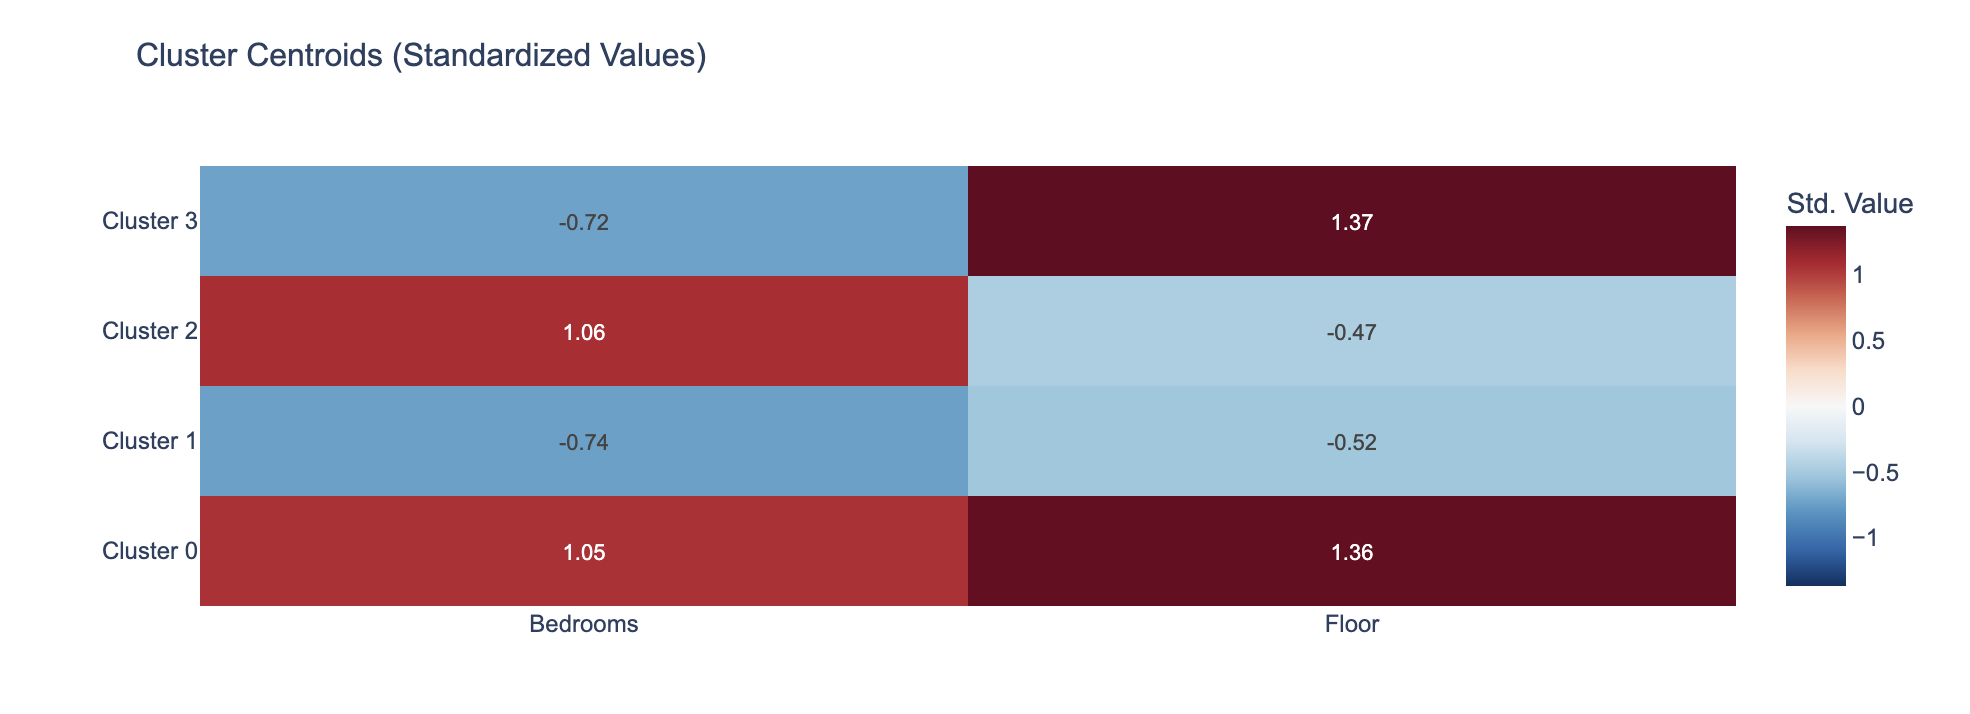
\includegraphics[width=\linewidth]{figures/centroids.png}
\caption{Cluster centroids --- standardised values.
The heatmap reveals a clean 2$\times$2 structure: Clusters 0 and 2 are
large-bedroom segments ($+$1.05--$+$1.06 SD) diverging sharply on floor
level ($+$1.36 vs.\ $-$0.47), while Clusters 1 and 3 are compact-bedroom
segments ($-$0.72--$-$0.74 SD) showing the same high/low floor split.
No centroid is near zero on both axes, confirming each cluster occupies
a distinct position in the feature space.}
\label{fig:centroids}
\end{figure}
\begin{figure}[H]
\centering
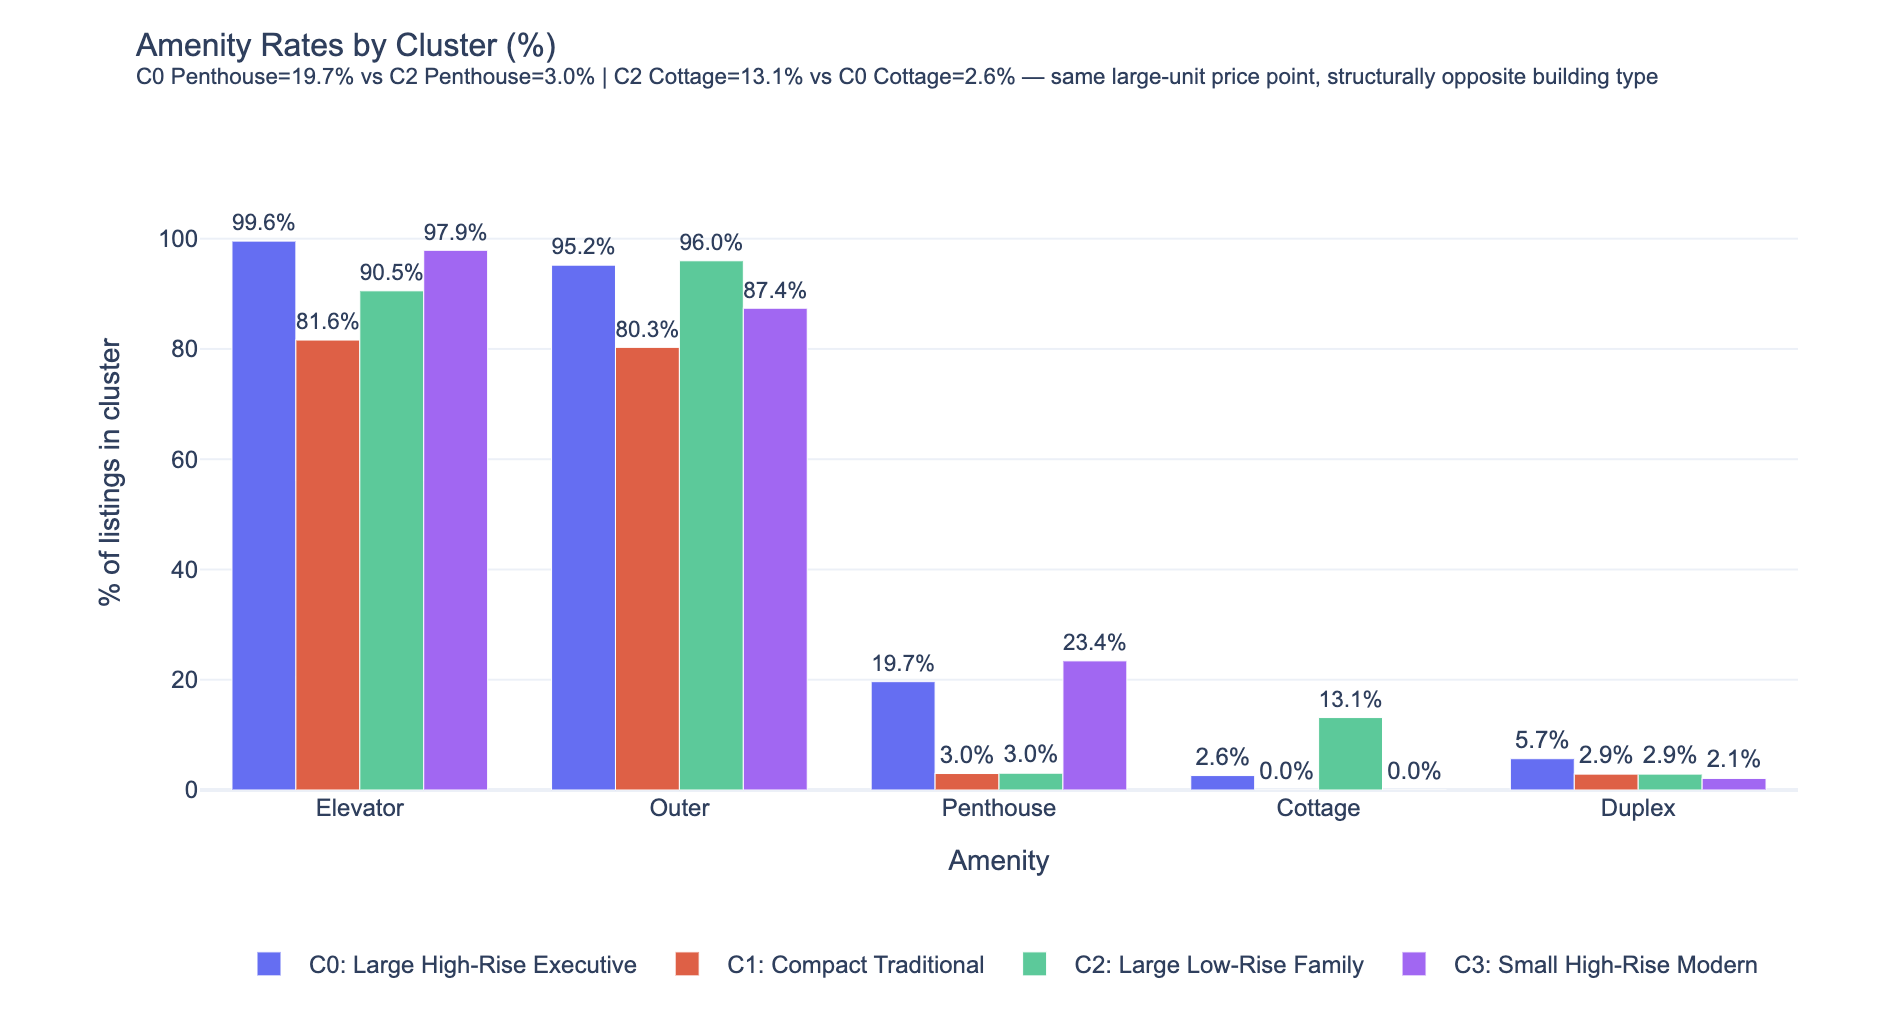
\includegraphics[width=\linewidth]{figures/amenities_bar.png}
\caption{Amenity rates by cluster (\%). Elevator and
Outer are near-universal across all segments and carry limited discriminating
power. The structurally opposite profiles of C0 and C2 are most visible in
Penthouse (19.7\% vs.\ 3.0\%) and Cottage (2.6\% vs.\ 13.1\%) --- two
clusters that share a similar price point but represent entirely different
building types, confirming that a blended model would conflate them.}
\label{fig:amenities}
\end{figure}


% ─── ANNEX 5 ─────────────────────────────────────────────────────────────────
\subsection*{Annex 5 --- Pricing Evidence}
\begin{figure}[H]
\centering
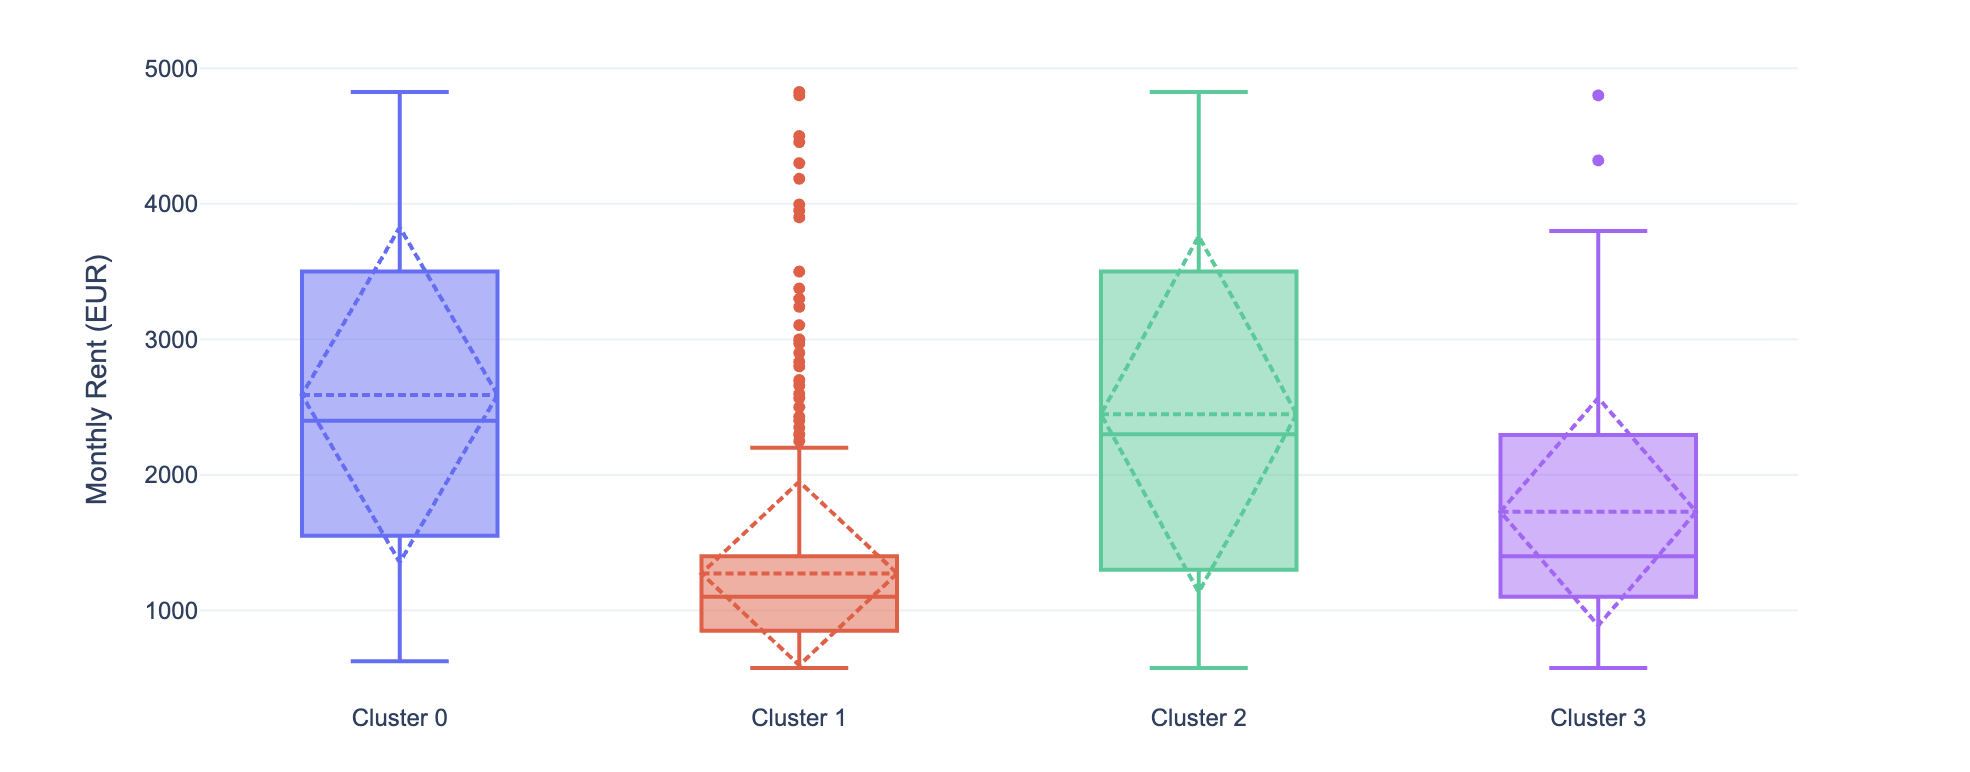
\includegraphics[width=\linewidth]{figures/monthly_rent_boxlot.png}
\caption{Monthly rent distribution by cluster (EUR).
C1 (Compact Traditional) is the tightest and lowest segment --- median
\euro{1,100}, IQR \euro{800}--\euro{1,250} --- confirming it as the
volume market. C0 and C2 share a similar median (\euro{2,300}--\euro{2,400})
but C2 carries a wider IQR, reflecting greater within-segment price
dispersion driven by floor-level variation. C3 (Compact High-Rise)
sits between the two price bands with a median near \euro{1,500},
occupying a structurally distinct mid-market position. The near-absence
of overlap between C1 and the remaining three clusters validates the
$K\!=\!4$ segmentation on economic grounds.}
\label{fig:rent_box}
\end{figure}

\begin{figure}[H]
\centering
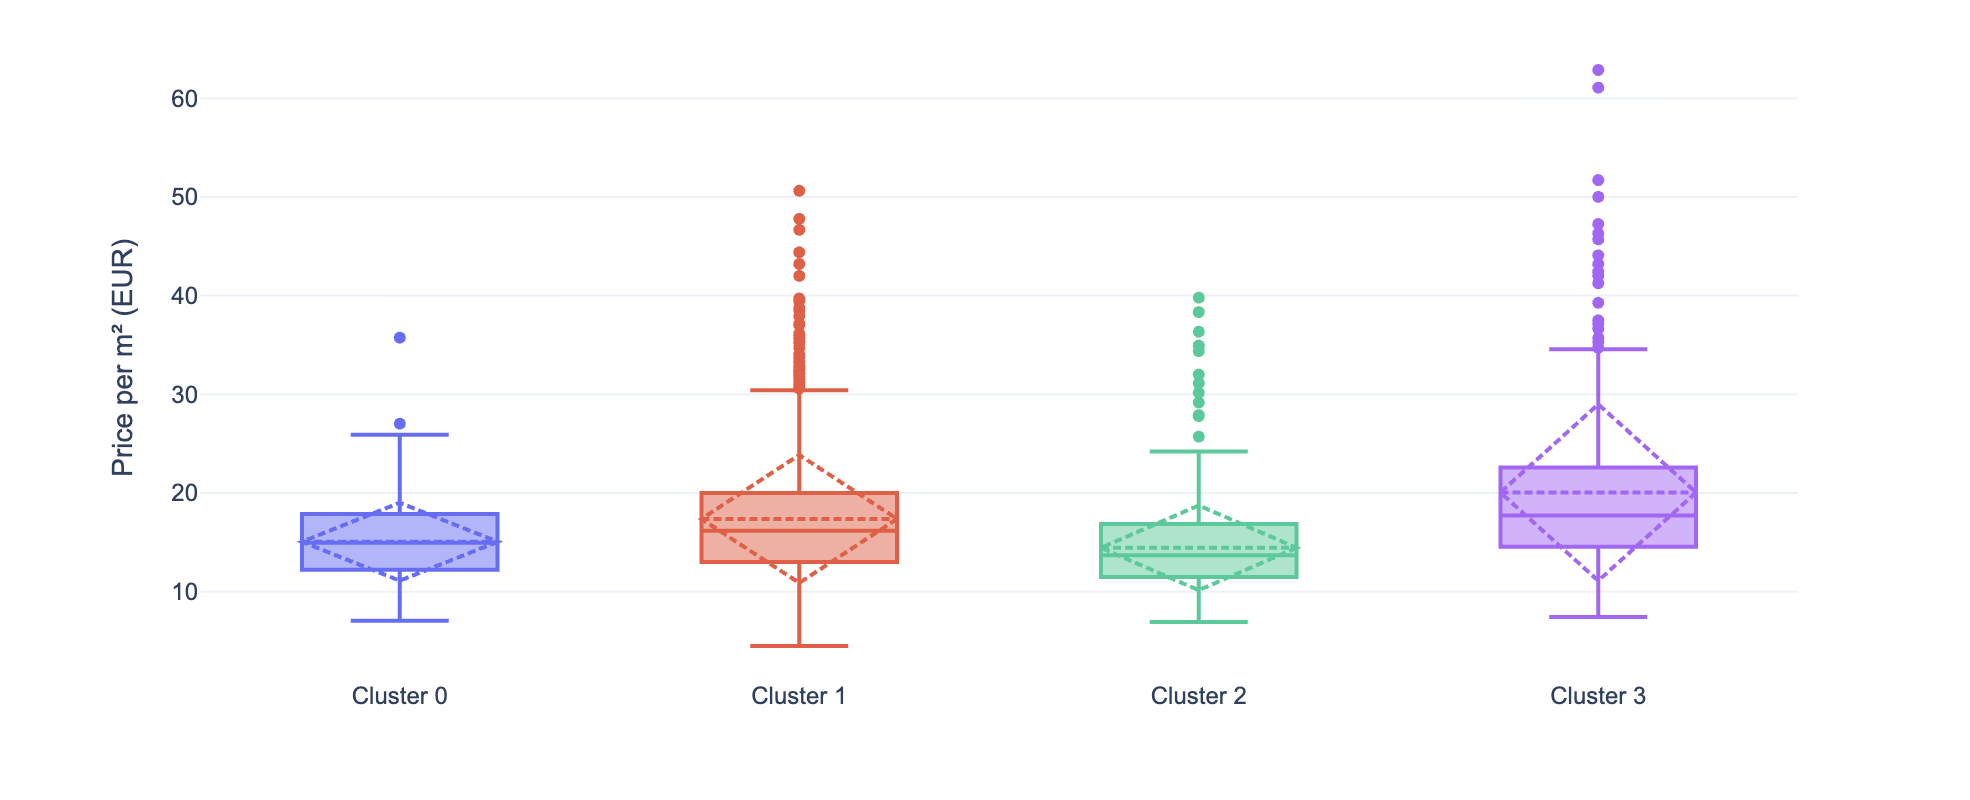
\includegraphics[width=\linewidth]{figures/price_per_sqm_boxplot.png}
\caption{Price per m$^2$ by cluster (EUR/m$^2$).
Medians converge across all four segments (\euro{13}--\euro{17}/m$^2$),
confirming that absolute rent differences are driven by unit size and
floor level rather than intrinsic price-per-m$^2$ premiums. C1 (Compact
Traditional) and C3 (Compact High-Rise) show the widest upper tails ---
consistent with the location-driven heterogeneity captured by the
Sq.Mt $\times$ District interaction terms in the regression model. The
convergence of medians across clusters provides the economic rationale
for modelling interactions rather than level shifts: it is \textit{where}
a square metre is located, not how many square metres there are, that
drives rent variation within the \seg{Compact Traditional} segment.}
\label{fig:sqm_box}
\end{figure}

\begin{figure}[H]
\centering
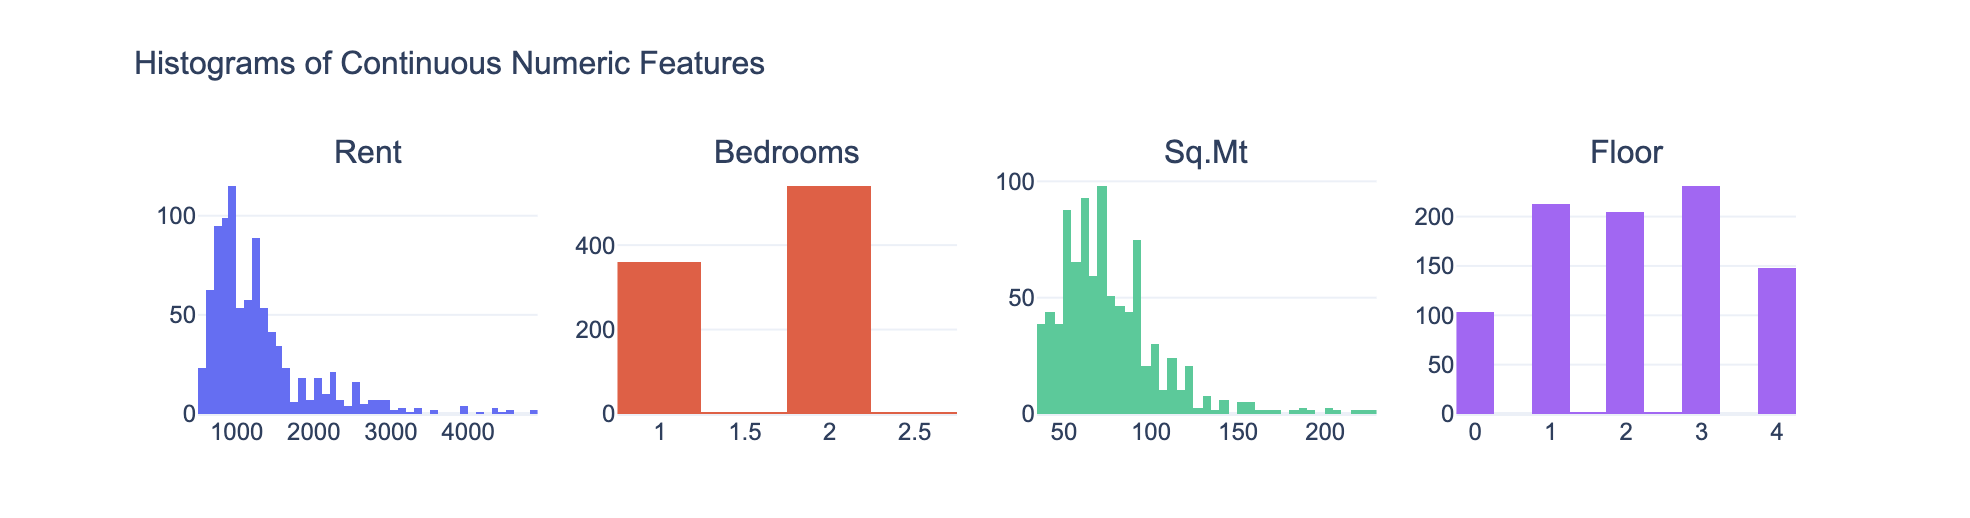
\includegraphics[width=\linewidth]{figures/histogram_continuous_regression.png}
\caption{Distribution of continuous numeric features after
outlier capping. Rent and Sq.Mt are right-skewed; Bedrooms concentrates at 1--2;
Floor peaks at levels 1--3.}
\label{fig:hist_cont}
\end{figure}

\begin{minipage}{\textwidth}
\begin{figure}[H]
\centering
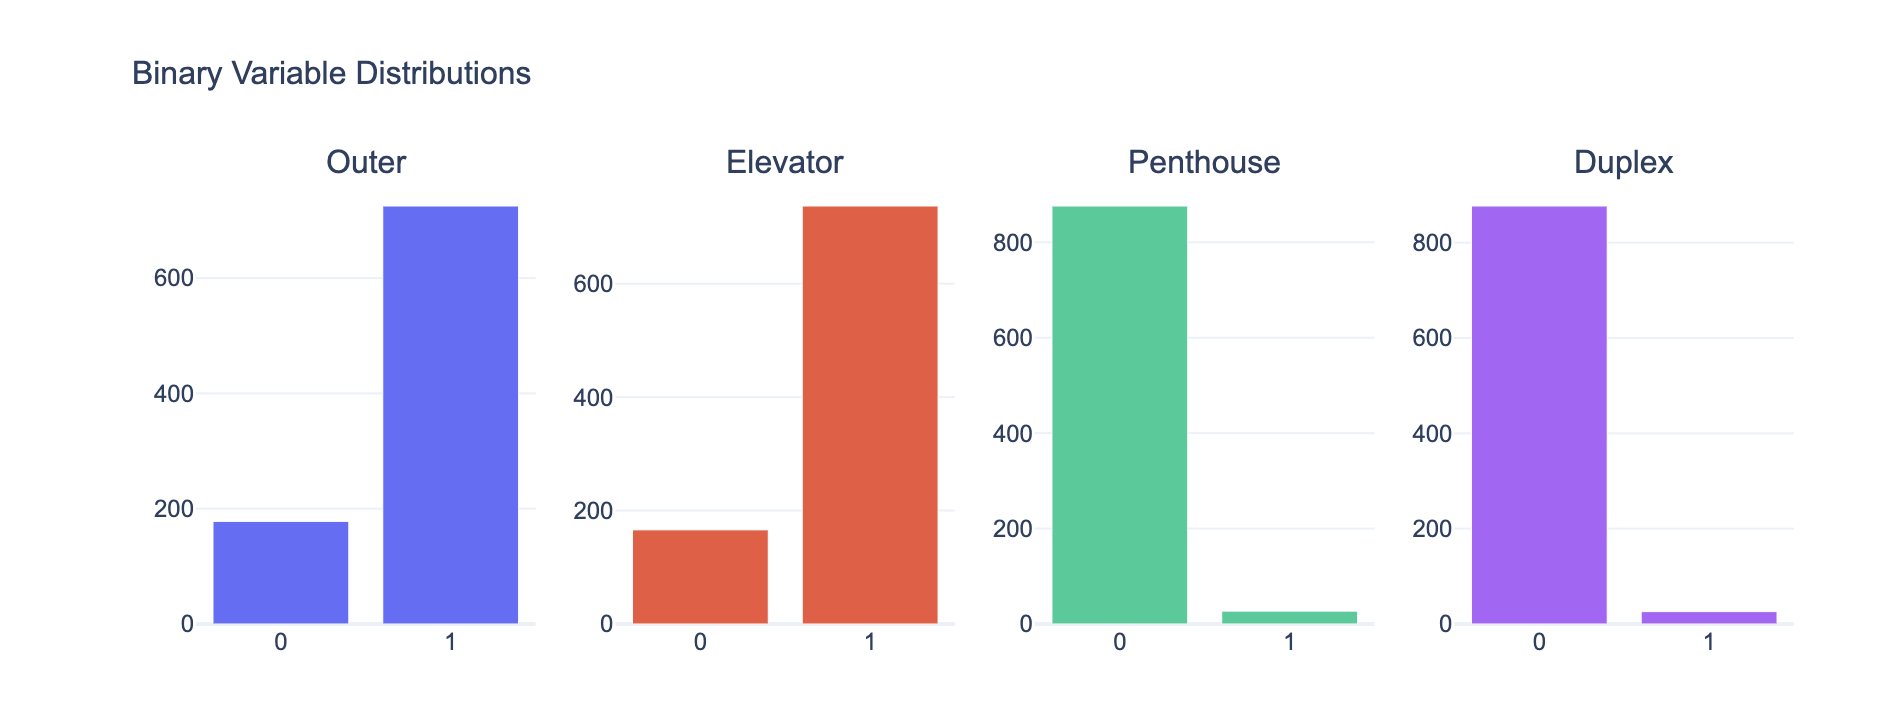
\includegraphics[width=\linewidth]{figures/histogram_binary_regression.png}
\caption{Distribution of binary amenity indicators.
Outer (80\%) and Elevator (82\%) are near-universal in \cluster{1}; Penthouse and Duplex
are rare ($<$5\%), justifying mode imputation at 0.}
\label{fig:hist_bin}
\end{figure}

\vspace{8pt}

\begin{table}[H]
\centering
\caption{District encoding --- before and after low-frequency grouping
(\textit{districts with $<$25 listings collapsed into ``Other''}).}
\label{tab:districts}
\small
\begin{tabular}{@{}lr@{\hspace{1.5cm}}lr@{}}
\toprule
\multicolumn{2}{c}{\textbf{Before grouping}} &
\multicolumn{2}{c}{\textbf{After grouping}} \\
\textbf{District} & \textbf{$n$} &
\textbf{District} & \textbf{$n$} \\
\midrule
Centro          & 196 & Centro          & 196 \\
Chamberí        &  90 & Chamberí        &  90 \\
Tetuán          &  86 & Tetuán          &  86 \\
Salamanca       &  81 & Salamanca       &  81 \\
Chamartín       &  75 & Chamartín       &  75 \\
Moncloa         &  41 & Moncloa         &  41 \\
Ciudad Lineal   &  39 & Ciudad Lineal   &  39 \\
San Blás        &  39 & San Blás        &  39 \\
Arganzuela      &  38 & Arganzuela      &  38 \\
Puente Vallecas &  34 & Puente Vallecas &  34 \\
Hortaleza       &  30 & Hortaleza       &  30 \\
Fuencarral      &  29 & Fuencarral      &  29 \\
Carabanchel     &  27 & Carabanchel     &  27 \\
Retiro          &  26 & Retiro          &  26 \\
\rowcolor{rowpink} Latina          &  17 & \textit{Other}  &  72 \\
\rowcolor{rowpink} Usera           &  17 & & \\
\rowcolor{rowpink} Vicálvaro       &  14 & & \\
\rowcolor{rowpink} Villa de Vallecas &  14 & & \\
\rowcolor{rowpink} Barajas         &  10 & & \\
\midrule
\textbf{Total}  & \textbf{903} & \textbf{Total} & \textbf{903} \\
\bottomrule
\end{tabular}
\end{table}
\end{minipage}

\begin{minipage}{\textwidth}
\begin{table}[H]
\centering
\caption{Initial OLS model --- full feature set before variable
selection ($n=406$). Rows highlighted in green are significant at $p<0.05$;
$\dagger$ denotes marginal significance ($p<0.10$).}
\label{tab:ols_initial}
\small
\begin{tabular}{@{}l r r r c r r@{}}
\toprule
\textbf{Variable} & \textbf{Coef.} & \textbf{Std.\ Err.} & \textbf{$t$} &
\textbf{$p$} & \textbf{95\% CI lower} & \textbf{95\% CI upper} \\
\midrule
\multicolumn{7}{@{}l}{\textit{Model fit: $R^2=0.628$,\; Adj.\ $R^2=0.607$,\;
$F(21,384)=30.80$,\; $p<0.001$,\; $n=406$,\; AIC=6061,\; BIC=6149}} \\[1pt]
const                       &   $-$2.50 & 141.93 &  $-$0.02 & 0.986         & $-$281.56 &  276.56 \\
Bedrooms                    &   $-$7.95 &  50.85 &  $-$0.16 & 0.876         & $-$107.93 &   92.04 \\
\rowcolor{passgreen}
Sq.Mt                       &    12.39  &   0.94 &   13.22  & $<$0.001\,*** &   10.55   &   14.24 \\
Floor                       &    21.08  &  17.33 &    1.22  & 0.225         & $-$12.99  &   55.14 \\
\rowcolor{passgreen}
Outer                       &   113.56  &  55.93 &    2.03  & 0.043\,*      &    3.60   &  223.52 \\
Elevator                    &    24.24  &  55.07 &    0.44  & 0.660         & $-$84.04  &  132.52 \\
Penthouse                   &    62.53  & 125.35 &    0.50  & 0.618         & $-$183.94 &  308.99 \\
Duplex                      &   162.32  & 162.35 &    1.00  & 0.318         & $-$156.89 &  481.54 \\
\midrule
\multicolumn{7}{@{}l}{\textit{District dummies (reference: Carabanchel)}} \\[2pt]
District\_Carabanchel       & $-$130.02 & 173.68 & $-$0.75  & 0.455         & $-$471.51 &  211.46 \\
\rowcolor{passgreen}
District\_Centro            &   382.80  & 118.14 &    3.24  & 0.001\,**     &  150.51   &  615.08 \\
District\_Chamartín         &   239.29  & 132.48 &    1.81  & 0.072\,$\dagger$ & $-$21.20 & 499.77 \\
\rowcolor{passgreen}
District\_Chamberí          &   376.78  & 128.65 &    2.93  & 0.004\,**     &  123.83   &  629.73 \\
District\_Ciudad Lineal     &     2.37  & 161.27 &    0.01  & 0.988         & $-$314.72 &  319.46 \\
District\_Fuencarral        &  $-$79.14 & 168.02 & $-$0.47  & 0.638         & $-$409.49 &  251.21 \\
District\_Hortaleza         &  $-$25.92 & 167.67 & $-$0.15  & 0.877         & $-$355.58 &  303.75 \\
District\_Moncloa           &   198.83  & 156.42 &    1.27  & 0.204         & $-$108.71 &  506.37 \\
District\_Other             & $-$240.48 & 135.29 & $-$1.78  & 0.076\,$\dagger$ & $-$506.47 & 25.52 \\
District\_Puente Vallecas   & $-$160.76 & 149.96 & $-$1.07  & 0.284         & $-$455.61 &  134.08 \\
District\_Retiro            &   264.45  & 153.95 &    1.72  & 0.087\,$\dagger$ & $-$38.24 & 567.13 \\
\rowcolor{passgreen}
District\_Salamanca         &   829.79  & 127.32 &    6.52  & $<$0.001\,*** &  579.46   & 1080.11 \\
District\_San Blás          & $-$222.13 & 150.03 & $-$1.48  & 0.140         & $-$517.10 &   72.85 \\
District\_Tetuán            &    73.75  & 129.17 &    0.57  & 0.568         & $-$180.21 &  327.71 \\
\midrule
\multicolumn{7}{@{}l}{\footnotesize $***\;p<0.001$;\quad $**\;p<0.01$;\quad
$*\;p<0.05$;\quad $\dagger\;p<0.10$. \quad Skew=1.685;\;
Kurtosis=9.307;\; DW=2.207.} \\
\bottomrule
\end{tabular}
\end{table}

\vspace{8pt}

\begin{table}[H]
\centering
\caption{OLS model after dropping clustering variables
(Bedrooms, Floor) --- rationale: within a single cluster these variables carry
minimal variance and add no meaningful predictive value ($n=406$).
Green = $p<0.05$;\; $\dagger$ = $p<0.10$.}
\label{tab:ols_dropped}
\small
\begin{tabular}{@{}l r r r c r r@{}}
\toprule
\textbf{Variable} & \textbf{Coef.} & \textbf{Std.\ Err.} & \textbf{$t$} &
\textbf{$p$} & \textbf{95\% CI lower} & \textbf{95\% CI upper} \\
\midrule
\multicolumn{7}{@{}l}{\textit{Model fit: $R^2=0.626$,\; Adj.\ $R^2=0.608$,\;
$F(19,386)=34.01$,\; $p<0.001$,\; $n=406$,\; AIC=6059,\; BIC=6139}} \\[1pt]
const                     &    18.23  & 129.35 &   0.14  & 0.888               & $-$236.09 &  272.55 \\
\rowcolor{passgreen}
Sq.Mt                     &    12.42  &   0.82 &  15.15  & $<$0.001\,***       &   10.81   &   14.03 \\
\rowcolor{passgreen}
Outer                     &   115.99  &  55.79 &   2.08  & 0.038\,*            &    6.30   &  225.68 \\
Elevator                  &    34.18  &  54.06 &   0.63  & 0.528               & $-$72.11  &  140.47 \\
Penthouse                 &    91.68  & 122.96 &   0.75  & 0.456               & $-$150.06 &  333.43 \\
Duplex                    &   170.67  & 162.10 &   1.05  & 0.293               & $-$148.04 &  489.38 \\
\midrule
\multicolumn{7}{@{}l}{\textit{District dummies (reference: Carabanchel)}} \\[2pt]
District\_Carabanchel     & $-$135.75 & 172.69 & $-$0.79 & 0.432               & $-$475.28 &  203.78 \\
\rowcolor{passgreen}
District\_Centro          &   385.41  & 117.98 &   3.27  & 0.001\,**           &  153.45   &  617.38 \\
District\_Chamartín       &   231.53  & 132.18 &   1.75  & 0.081\,$\dagger$    & $-$28.35  &  491.41 \\
\rowcolor{passgreen}
District\_Chamberí        &   374.00  & 128.53 &   2.91  & 0.004\,**           &  121.31   &  626.70 \\
District\_Ciudad Lineal   &    14.32  & 160.84 &   0.09  & 0.929               & $-$301.90 &  330.55 \\
District\_Fuencarral      &  $-$89.65 & 166.91 & $-$0.54 & 0.592               & $-$417.80 &  238.51 \\
District\_Hortaleza       &  $-$29.87 & 167.46 & $-$0.18 & 0.859               & $-$359.12 &  299.39 \\
District\_Moncloa         &   185.90  & 155.77 &   1.19  & 0.233               & $-$120.37 &  492.17 \\
District\_Other           & $-$239.30 & 134.78 & $-$1.78 & 0.077\,$\dagger$    & $-$504.29 &   25.69 \\
District\_Puente Vallecas & $-$173.88 & 148.92 & $-$1.17 & 0.244               & $-$466.67 &  118.92 \\
District\_Retiro          &   256.59  & 153.54 &   1.67  & 0.095\,$\dagger$    & $-$45.29  &  558.47 \\
\rowcolor{passgreen}
District\_Salamanca       &   828.02  & 127.21 &   6.51  & $<$0.001\,***       &  577.91   & 1078.14 \\
District\_San Blás        & $-$220.92 & 149.88 & $-$1.47 & 0.141               & $-$515.60 &   73.77 \\
District\_Tetuán          &    76.15  & 128.78 &   0.59  & 0.555               & $-$177.05 &  329.34 \\
\midrule
\multicolumn{7}{@{}l}{\footnotesize $***\;p<0.001$;\quad $**\;p<0.01$;\quad
$*\;p<0.05$;\quad $\dagger\;p<0.10$.\quad Skew=1.649;\;
Kurtosis=9.019;\; DW=2.205.} \\
\bottomrule
\end{tabular}
\end{table}
\end{minipage}

\begin{minipage}{\textwidth}
\begin{table}[H]
\centering
\caption{Variance Inflation Factors after dropping
clustering variables. VIF $\geq5$ flagged in amber; no variable exceeds the
hard threshold of 10.}
\label{tab:vif_reg}
\small
\begin{tabular}{@{}l r@{}}
\toprule
\textbf{Variable} & \textbf{VIF} \\
\midrule
\multicolumn{2}{@{}l}{\textit{Physical features}} \\[1pt]
\rowcolor{orange!20} Sq.Mt                    & 8.68 \\
\rowcolor{orange!20} Outer                    & 5.90 \\
\rowcolor{orange!20} Elevator                 & 5.23 \\
Penthouse                & 1.07 \\
Duplex                   & 1.08 \\
\midrule
\multicolumn{2}{@{}l}{\textit{District dummies}} \\[2pt]
District\_Centro         & 2.75 \\
District\_Salamanca      & 2.18 \\
District\_Chamartín      & 1.80 \\
District\_Chamberí       & 1.70 \\
District\_Tetuán         & 1.65 \\
District\_Other          & 1.61 \\
District\_San Blás       & 1.45 \\
District\_Retiro         & 1.42 \\
District\_Moncloa        & 1.32 \\
District\_Puente Vallecas & 1.29 \\
District\_Ciudad Lineal  & 1.29 \\
District\_Fuencarral     & 1.28 \\
District\_Hortaleza      & 1.25 \\
District\_Carabanchel    & 1.17 \\
\midrule
\multicolumn{2}{@{}l}{\footnotesize Threshold: VIF $<5$ acceptable;\;
VIF $\geq10$ requires removal.} \\
\bottomrule
\end{tabular}
\end{table}

\vspace{8pt}

\begin{table}[H]
\centering
\caption{Final OLS model --- Sq.Mt $\times$ District
interactions ($n=406$, $df_{\text{model}}=10$). All retained predictors
significant at $p<0.05$. Condition number = 429, well below the
collinearity threshold of 1{,}000.}
\label{tab:ols_final}
\small
\begin{tabular}{@{}l r r r c r r@{}}
\toprule
\textbf{Variable} & \textbf{Coef.} & \textbf{Std.\ Err.} & \textbf{$t$} &
\textbf{$p$} & \textbf{95\% CI lower} & \textbf{95\% CI upper} \\
\midrule
\multicolumn{7}{@{}l}{\textit{Model fit: $R^2=0.644$,\; Adj.\ $R^2=0.635$,\;
$F(10,395)=71.53$,\; $p<0.001$,\; $n=406$,\; AIC=6020,\; BIC=6065}} \\[1pt]
\multicolumn{7}{@{}l}{\textit{Base predictors}} \\[2pt]
\rowcolor{passgreen} const                    & 375.39  &  63.26 &  5.94 & $<$0.001\,*** &  251.04 &  499.75 \\
\rowcolor{passgreen} Sq.Mt                    &   7.38  &   0.95 &  7.78 & $<$0.001\,*** &    5.52 &    9.25 \\
\rowcolor{passgreen} Outer                    & 107.27  &  51.84 &  2.07 & 0.039\,*      &    5.37 &  209.18 \\
\rowcolor{passgreen} District\_Other          & $-$214.98 & 79.51 & $-$2.70 & 0.007\,** & $-$371.30 & $-$58.65 \\
\rowcolor{passgreen} District\_Puente Vallecas & $-$199.91 & 99.25 & $-$2.01 & 0.045\,* & $-$395.03 & $-$4.80 \\
\midrule
\multicolumn{7}{@{}l}{\textit{Sq.Mt $\times$ District interactions
(additional \euro{} per m$^2$ vs.\ baseline)}} \\[2pt]
\rowcolor{passgreen} SqMt $\times$ Centro     & $+$6.03  & 0.73 & 8.31  & $<$0.001\,*** & 4.60  &  7.46 \\
\rowcolor{passgreen} SqMt $\times$ Chamartín  & $+$3.79  & 0.99 & 3.85  & $<$0.001\,*** & 1.85  &  5.73 \\
\rowcolor{passgreen} SqMt $\times$ Chamberí   & $+$5.78  & 0.96 & 6.02  & $<$0.001\,*** & 3.90  &  7.68 \\
\rowcolor{passgreen} SqMt $\times$ Moncloa    & $+$3.22  & 1.41 & 2.28  & 0.023\,*      & 0.44  &  5.99 \\
\rowcolor{passgreen} SqMt $\times$ Retiro     & $+$4.26  & 1.20 & 3.57  & $<$0.001\,*** & 1.92  &  6.61 \\
\rowcolor{passgreen} SqMt $\times$ Salamanca  & $+$10.85 & 0.83 & 13.12 & $<$0.001\,*** & 9.22  & 12.47 \\
\midrule
\multicolumn{7}{@{}l}{\footnotesize $***\;p<0.001$;\quad $**\;p<0.01$;\quad
$*\;p<0.05$.\quad Skew=1.738;\; Kurtosis=9.250;\; DW=2.192;\;
Cond.\ No.=429.} \\
\bottomrule
\end{tabular}
\end{table}
\end{minipage}

\begin{minipage}{\textwidth}
\begin{figure}[H]
\centering
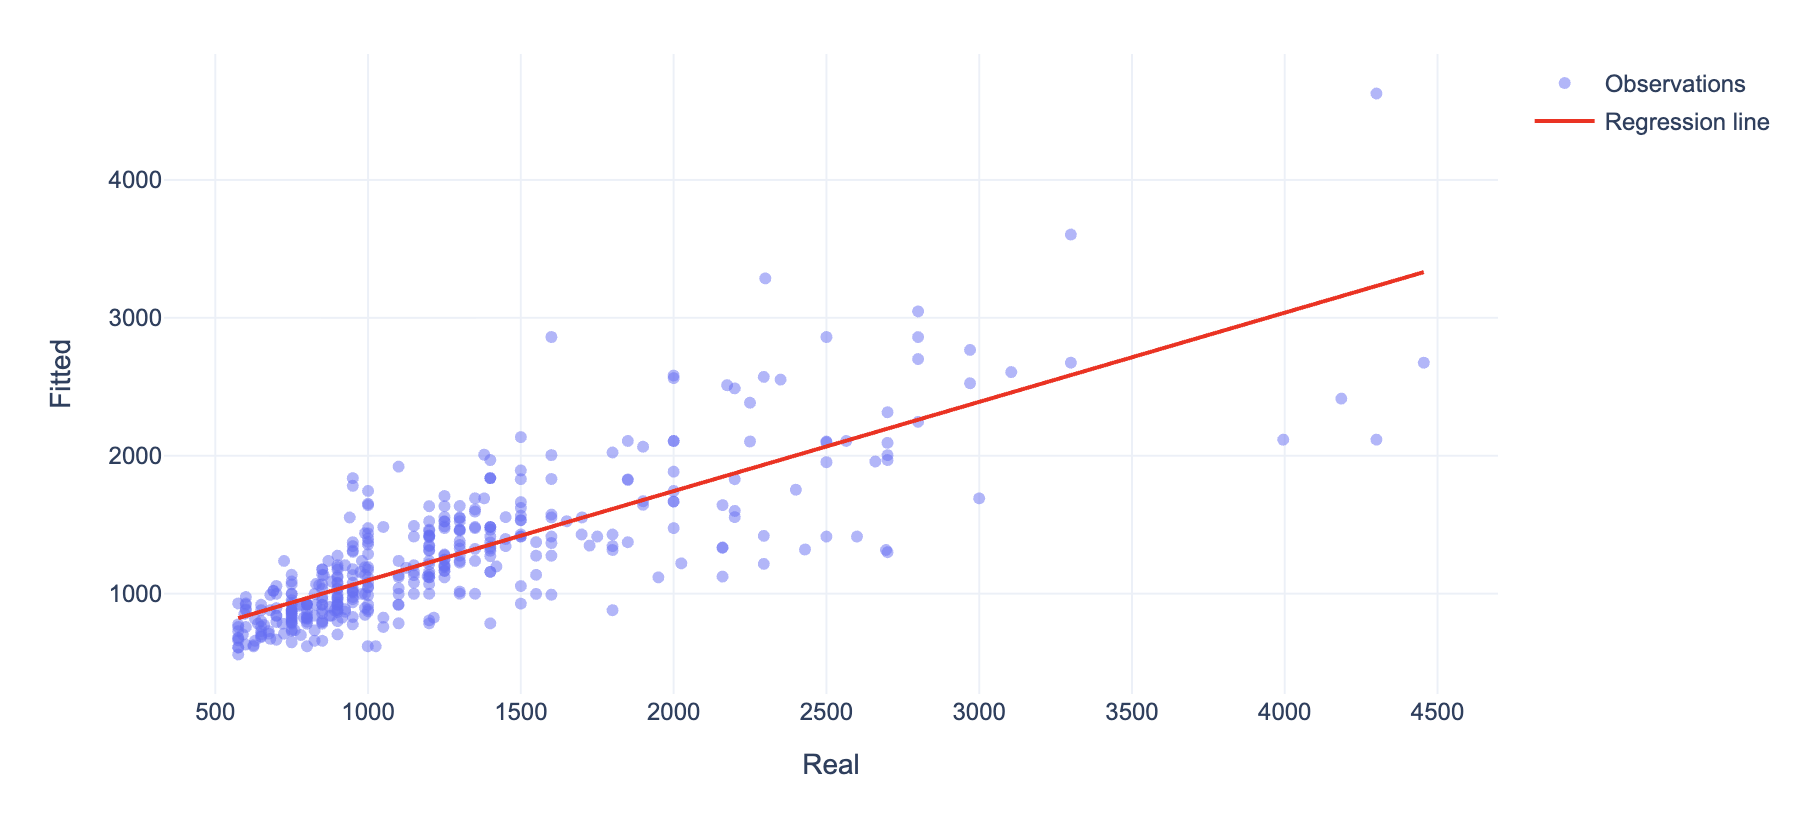
\includegraphics[width=\linewidth]{figures/real_vs_fitted_train.png}
\caption{Real vs.\ fitted values --- training set ($n\!=\!406$). Points cluster tightly along the diagonal… Scatter above €2,000 reflects high-specification properties whose prestige-street effects lie outside the model's observable features.}
\label{fig:rvf_train}
\end{figure}
\vspace{8pt}
\begin{figure}[H]
\centering
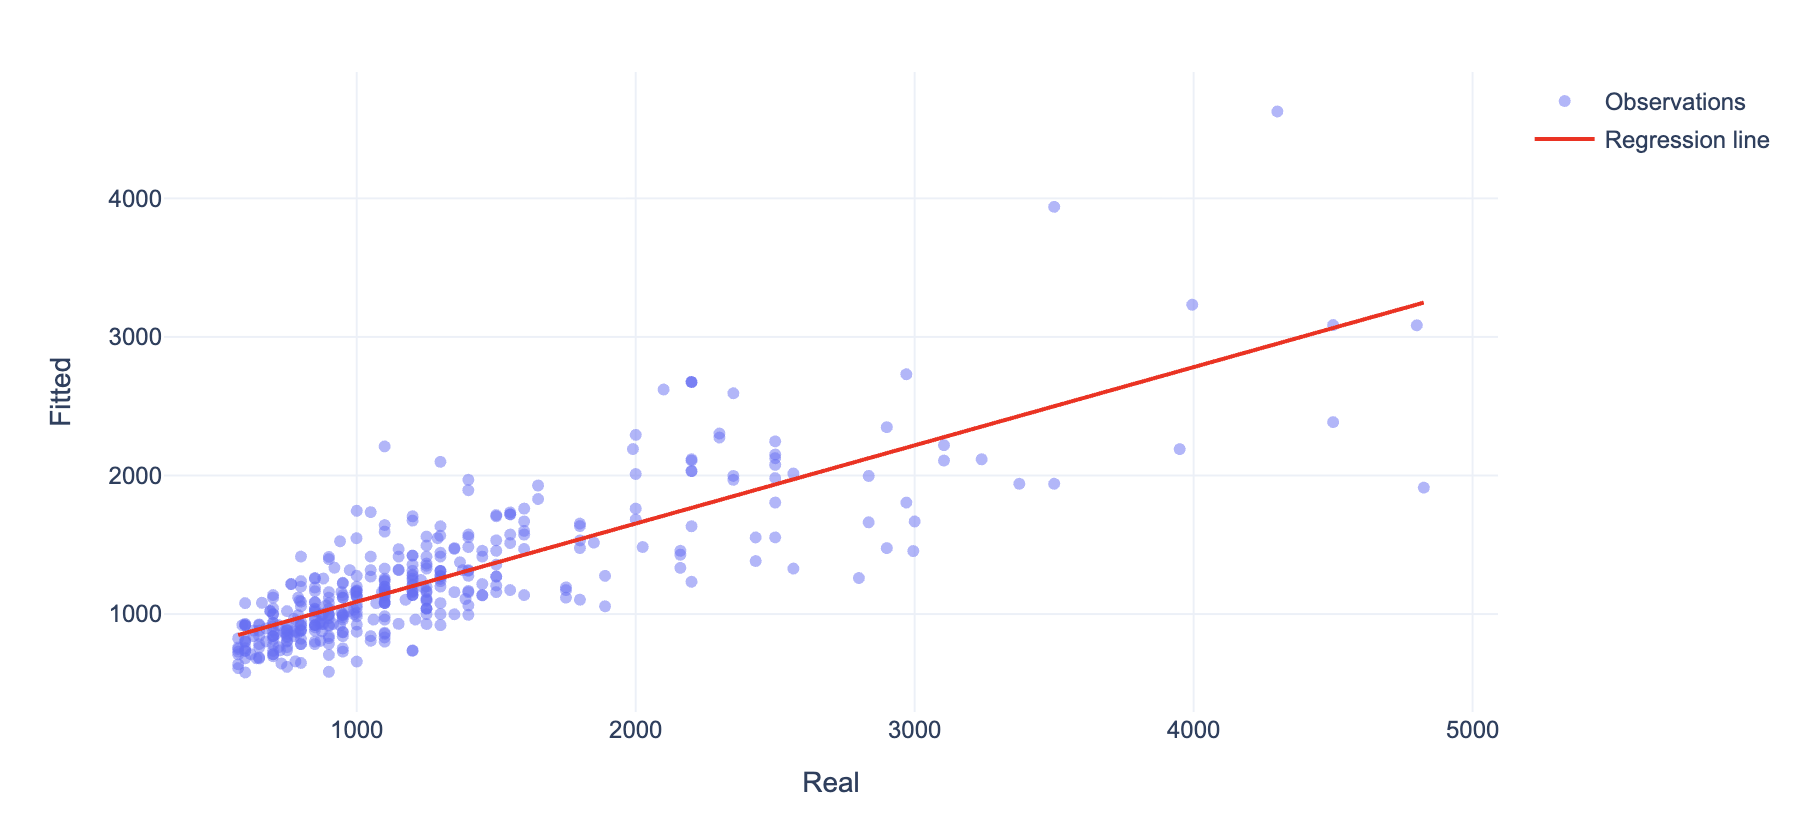
\includegraphics[width=\linewidth]{figures/real_vs_fitted_test.png}
\caption{Real vs.\ fitted values --- test set ($n=203$).
The regression line maintains a consistent slope with no systematic tilt, confirming the model generalises to unseen data. Scatter increases above \euro{2{,}000}, where prestige-street effects and interior specification push actual rents beyond what district and square meters alone can explain.}
\label{fig:rvf_test}
\end{figure}
\end{minipage}

\begin{minipage}{\textwidth}
\begin{figure}[H]
\centering
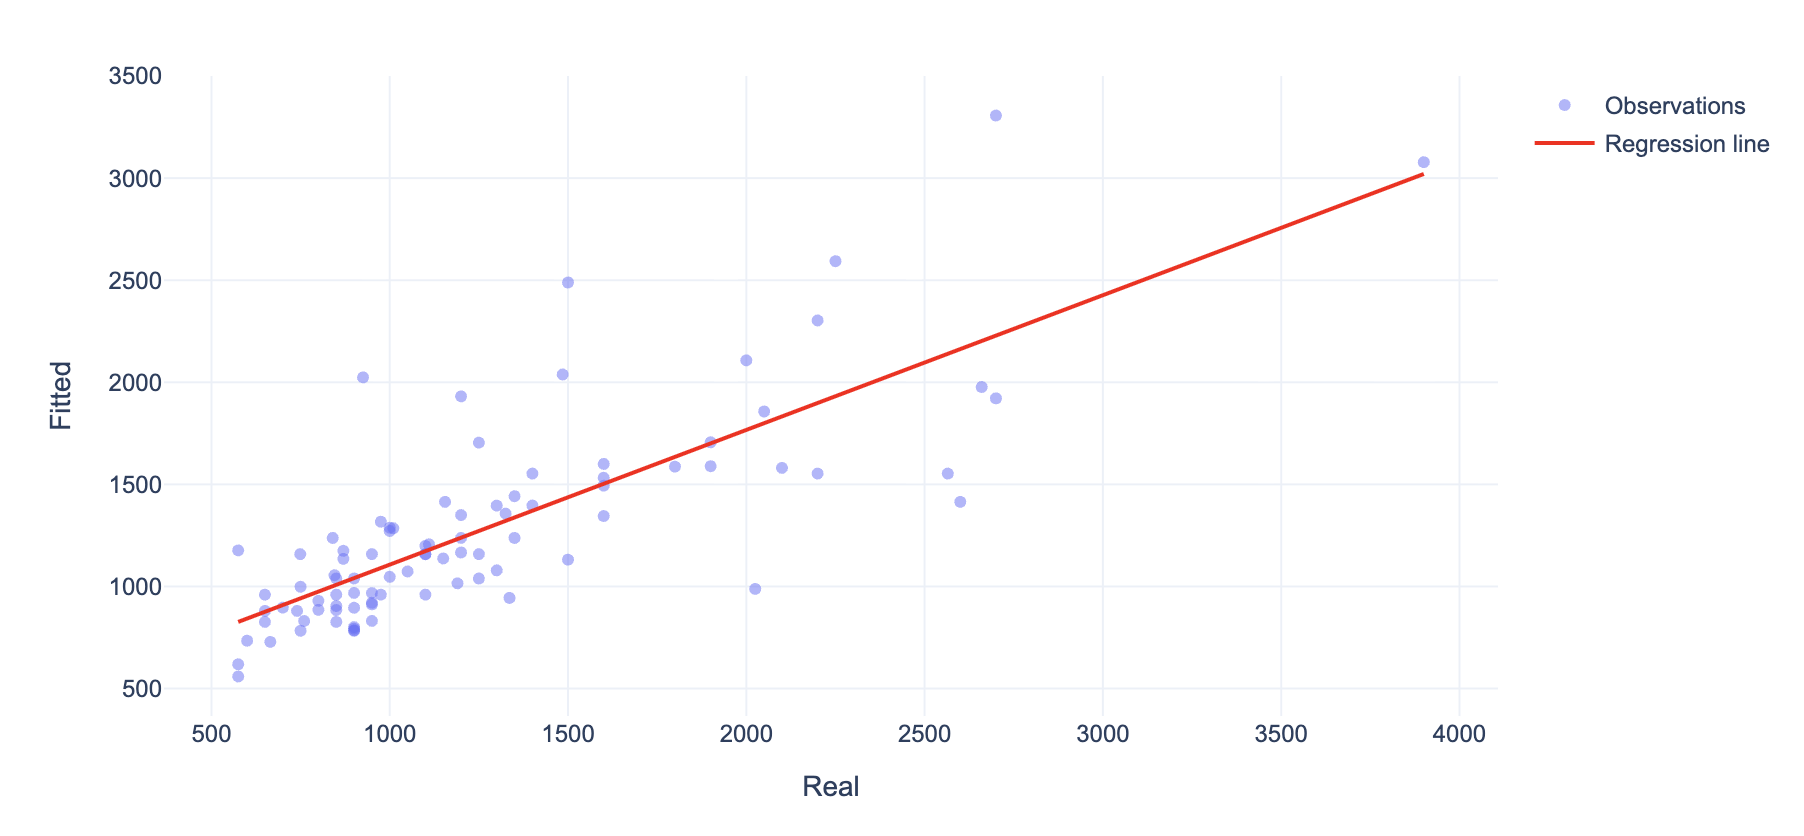
\includegraphics[width=\linewidth]{figures/real_vs_fitted_reserved.png}
\caption{Real vs.\ fitted values --- reserved hold-out
($n=41$). Despite never being seen at any stage of training or feature
selection, the regression slope remains consistent with the training and test splits. The two high-leverage points above \euro{2{,}500} confirm the upper-end under-prediction pattern is structural, not a product of the training sample.}
\label{fig:rvf_reserved}
\end{figure}
\vspace{8pt}

\begin{figure}[H]
\centering
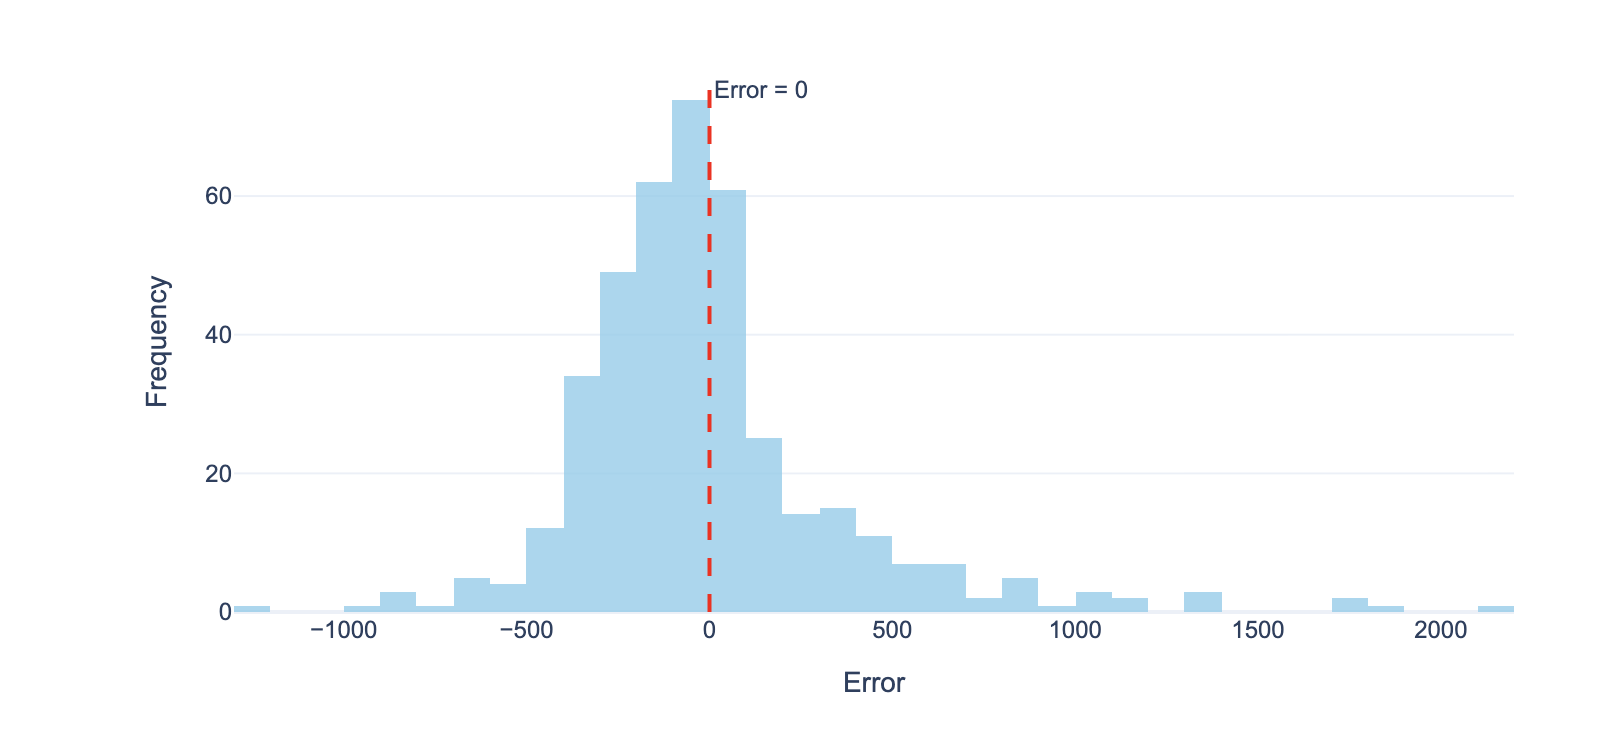
\includegraphics[width=\linewidth]{figures/residuals_train.png}
\caption{Residual distribution --- training set ($n=162$).
The distribution centers tightly on zero with no systematic shift,
confirming the model is unbiased across the majority of the segment.
The right tail extending to \euro{$+$2{,}100} and the near-absence of
a symmetric left tail indicate the model under-predicts selectively at
the top end --- consistent with the Skew = 1.738 and Kurtosis = 9.250
reported in the OLS diagnostics.}
\label{fig:resid_train}
\end{figure}
\end{minipage}

\begin{minipage}{\textwidth}
\begin{figure}[H]
\centering
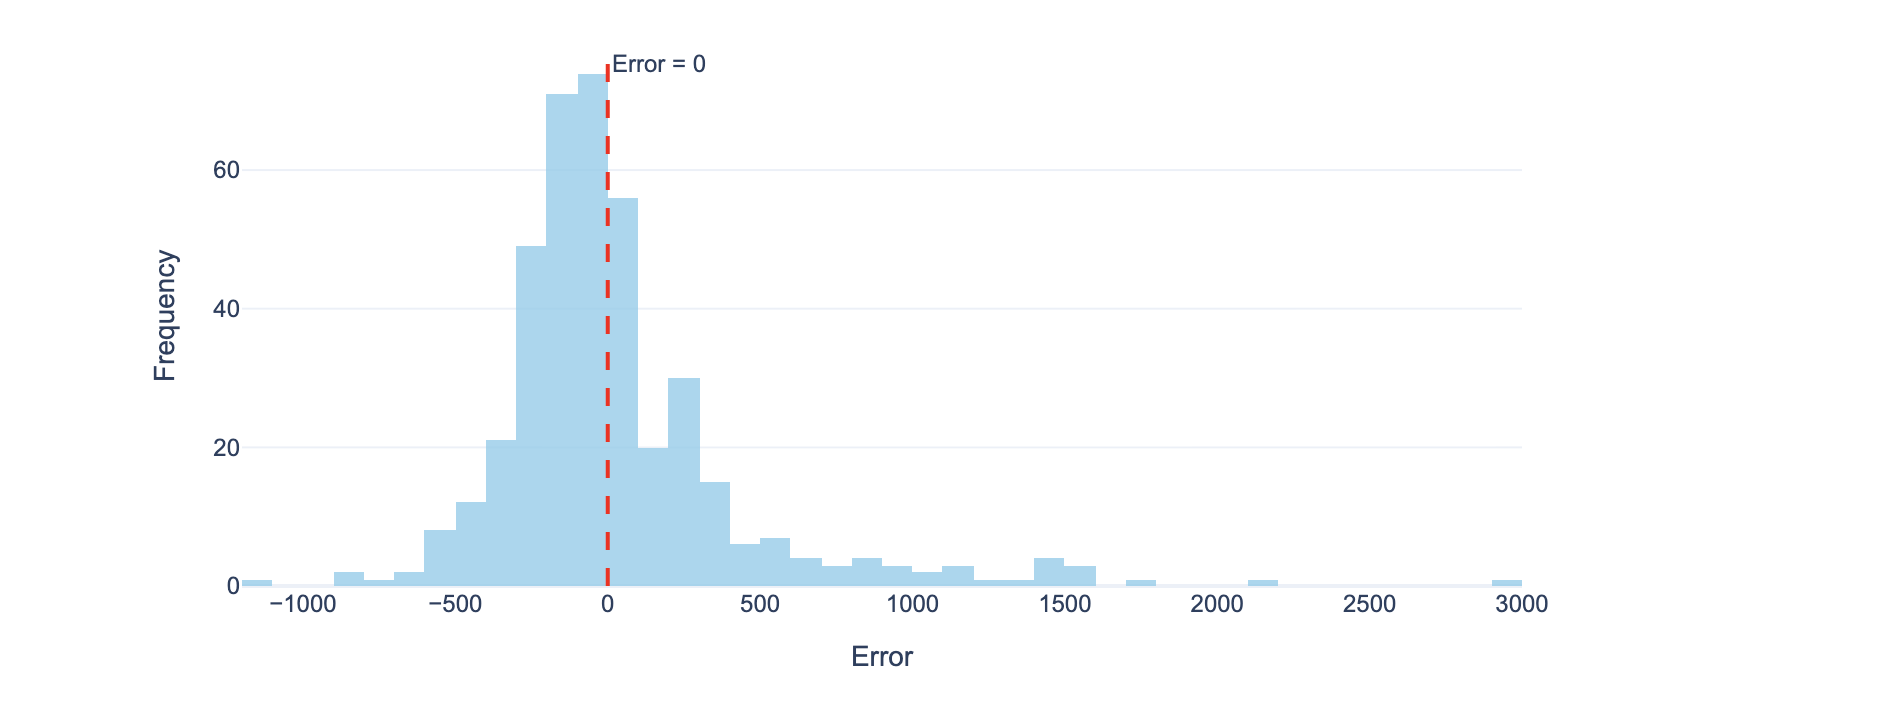
\includegraphics[width=\linewidth]{figures/residuals_test.png}
\caption{Residual distribution --- test set ($n=203$).
The distribution mirrors the training pattern: mass concentrated within
\euro{$\pm$500} of zero with no leftward shift, indicating the model
does not systematically over-predict on unseen data. The isolated bars
beyond \euro{$+$1{,}500} reinforce that large errors are confined to a
handful of outlier properties rather than distributed across the segment,
which explains the RMSE--MAE gap without inflating the typical error.}
\label{fig:resid_test}
\end{figure}
\vspace{8pt}
\begin{figure}[H]
\centering
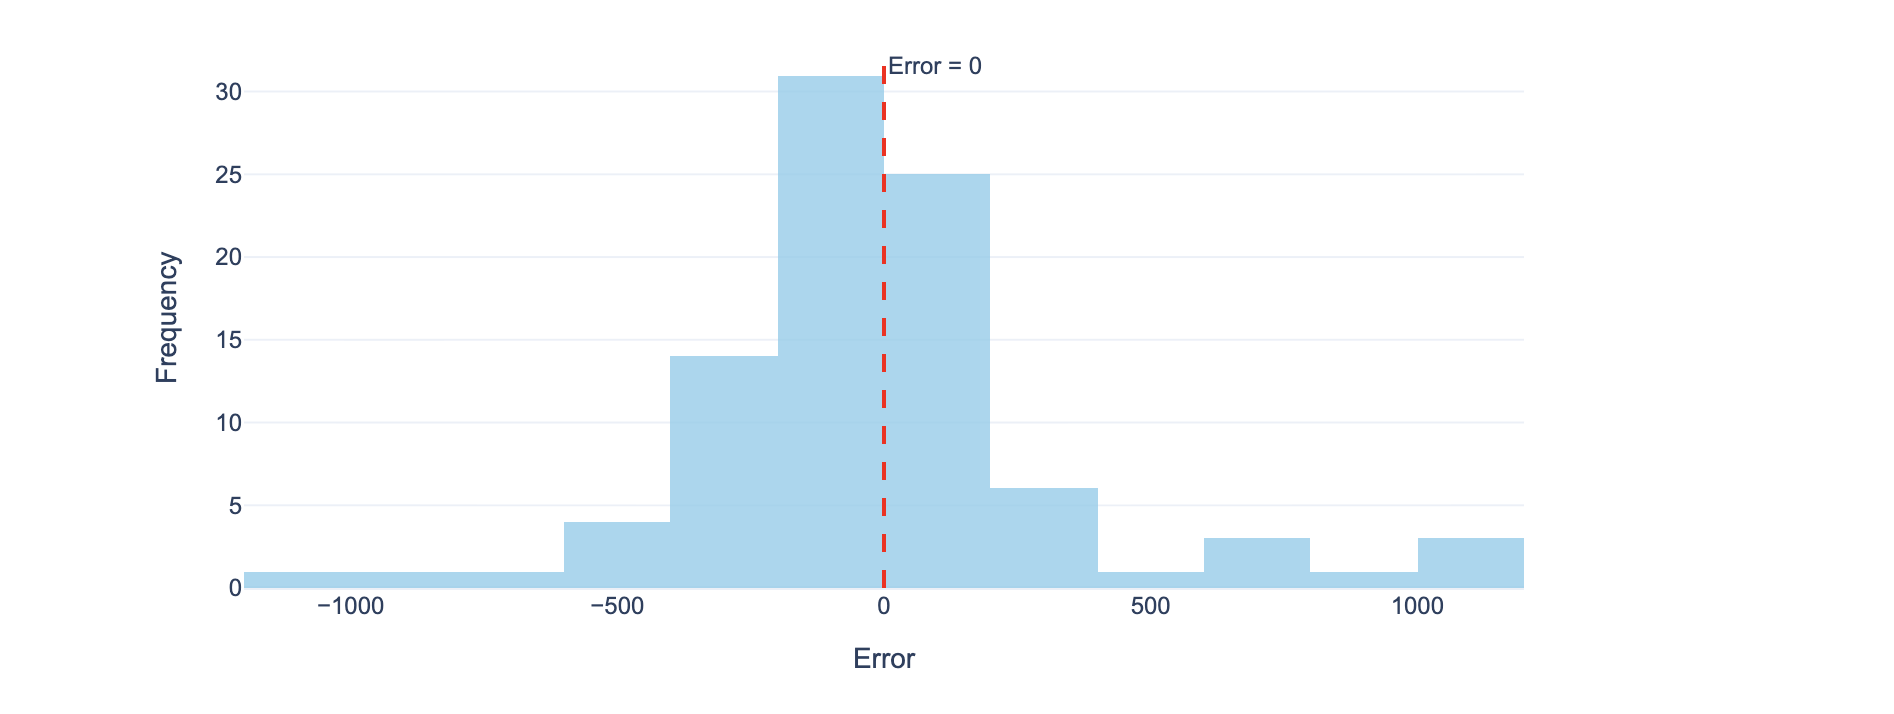
\includegraphics[width=\linewidth]{figures/residuals_reserved.png}
\caption{Residual distribution --- reserved hold-out.
The bulk of errors concentrates within \euro{$\pm$300} of zero with no
systematic bias, confirming the model does not persistently over- or
under-predict. The right tail extending to \euro{$+$2{,}100} reflects the
same structural ceiling identified in the real vs.\ fitted plots: a small
number of high-specification properties whose rents exceed what observable
features can explain.}
\label{fig:resid_reserved}
\end{figure}
\end{minipage}
\end{document}